% Options for packages loaded elsewhere
\PassOptionsToPackage{unicode}{hyperref}
\PassOptionsToPackage{hyphens}{url}
\documentclass[
  11pt,
]{article}
\usepackage{xcolor}
\usepackage[margin=22mm]{geometry}
\usepackage{amsmath,amssymb}
\setcounter{secnumdepth}{-\maxdimen} % remove section numbering
\usepackage{iftex}
\ifPDFTeX
  \usepackage[T1]{fontenc}
  \usepackage[utf8]{inputenc}
  \usepackage{textcomp} % provide euro and other symbols
\else % if luatex or xetex
  \usepackage{unicode-math} % this also loads fontspec
  \defaultfontfeatures{Scale=MatchLowercase}
  \defaultfontfeatures[\rmfamily]{Ligatures=TeX,Scale=1}
\fi
\usepackage{lmodern}
\ifPDFTeX\else
  % xetex/luatex font selection
\fi
% Use upquote if available, for straight quotes in verbatim environments
\IfFileExists{upquote.sty}{\usepackage{upquote}}{}
\IfFileExists{microtype.sty}{% use microtype if available
  \usepackage[]{microtype}
  \UseMicrotypeSet[protrusion]{basicmath} % disable protrusion for tt fonts
}{}
\makeatletter
\@ifundefined{KOMAClassName}{% if non-KOMA class
  \IfFileExists{parskip.sty}{%
    \usepackage{parskip}
  }{% else
    \setlength{\parindent}{0pt}
    \setlength{\parskip}{6pt plus 2pt minus 1pt}}
}{% if KOMA class
  \KOMAoptions{parskip=half}}
\makeatother
\usepackage{graphicx}
\makeatletter
\newsavebox\pandoc@box
\newcommand*\pandocbounded[1]{% scales image to fit in text height/width
  \sbox\pandoc@box{#1}%
  \Gscale@div\@tempa{\textheight}{\dimexpr\ht\pandoc@box+\dp\pandoc@box\relax}%
  \Gscale@div\@tempb{\linewidth}{\wd\pandoc@box}%
  \ifdim\@tempb\p@<\@tempa\p@\let\@tempa\@tempb\fi% select the smaller of both
  \ifdim\@tempa\p@<\p@\scalebox{\@tempa}{\usebox\pandoc@box}%
  \else\usebox{\pandoc@box}%
  \fi%
}
% Set default figure placement to htbp
\def\fps@figure{htbp}
\makeatother
\setlength{\emergencystretch}{3em} % prevent overfull lines
\providecommand{\tightlist}{%
  \setlength{\itemsep}{0pt}\setlength{\parskip}{0pt}}
\usepackage{bookmark}
\IfFileExists{xurl.sty}{\usepackage{xurl}}{} % add URL line breaks if available
\urlstyle{same}
\hypersetup{
  hidelinks,
  pdfcreator={LaTeX via pandoc}}

\author{}
\date{}

\newfontfamily\ReaderSymbols{seguisym.ttf}[Path=C:/Windows/Fonts/]
\makeatletter
\let\ReaderOriginalAnchorStart\hyper@anchorstart
\let\ReaderOriginalAnchorEnd\hyper@anchorend
\expandafter\def\csname ReaderAliases@section*.1\endcsname{\ReaderOriginalAnchorStart{causal-kernels-initial-data-and-short-time-geometry}\ReaderOriginalAnchorEnd}
\expandafter\def\csname ReaderAliases@section*.2\endcsname{\ReaderOriginalAnchorStart{AN03-WHK-001}\ReaderOriginalAnchorEnd\begingroup\def\@currentHref{AN03-WHK-001}\label{AN03-WHK-001}\endgroup\ReaderOriginalAnchorStart{an03-whk-001-conventions-and-the-causal-distribution-problem}\ReaderOriginalAnchorEnd\begingroup\def\@currentHref{an03-whk-001-conventions-and-the-causal-distribution-problem}\label{an03-whk-001-conventions-and-the-causal-distribution-problem}\endgroup\ReaderOriginalAnchorStart{1-conventions-and-the-causal-distribution-problem}\ReaderOriginalAnchorEnd\begingroup\def\@currentHref{1-conventions-and-the-causal-distribution-problem}\label{1-conventions-and-the-causal-distribution-problem}\endgroup\ReaderOriginalAnchorStart{conventions-and-the-causal-distribution-problem}\ReaderOriginalAnchorEnd}
\expandafter\def\csname ReaderAliases@section*.6\endcsname{\ReaderOriginalAnchorStart{AN03-WHK-002}\ReaderOriginalAnchorEnd\begingroup\def\@currentHref{AN03-WHK-002}\label{AN03-WHK-002}\endgroup\ReaderOriginalAnchorStart{an03-whk-002-a-laplace-calculation-that-constructs-the-whole-family}\ReaderOriginalAnchorEnd\begingroup\def\@currentHref{an03-whk-002-a-laplace-calculation-that-constructs-the-whole-family}\label{an03-whk-002-a-laplace-calculation-that-constructs-the-whole-family}\endgroup\ReaderOriginalAnchorStart{2-a-laplace-calculation-that-constructs-the-whole-family}\ReaderOriginalAnchorEnd\begingroup\def\@currentHref{2-a-laplace-calculation-that-constructs-the-whole-family}\label{2-a-laplace-calculation-that-constructs-the-whole-family}\endgroup\ReaderOriginalAnchorStart{a-laplace-calculation-that-constructs-the-whole-family}\ReaderOriginalAnchorEnd}
\expandafter\def\csname ReaderAliases@section*.21\endcsname{\ReaderOriginalAnchorStart{the-full-damping-branch-and-continuation-maps}\ReaderOriginalAnchorEnd}
\expandafter\def\csname ReaderAliases@section*.27\endcsname{\ReaderOriginalAnchorStart{AN03-WHK-003}\ReaderOriginalAnchorEnd\begingroup\def\@currentHref{AN03-WHK-003}\label{AN03-WHK-003}\endgroup\ReaderOriginalAnchorStart{an03-whk-003-cone-formulas-and-exact-recursion}\ReaderOriginalAnchorEnd\begingroup\def\@currentHref{an03-whk-003-cone-formulas-and-exact-recursion}\label{an03-whk-003-cone-formulas-and-exact-recursion}\endgroup\ReaderOriginalAnchorStart{3-cone-formulas-and-exact-recursion}\ReaderOriginalAnchorEnd\begingroup\def\@currentHref{3-cone-formulas-and-exact-recursion}\label{3-cone-formulas-and-exact-recursion}\endgroup\ReaderOriginalAnchorStart{cone-formulas-and-exact-recursion}\ReaderOriginalAnchorEnd}
\expandafter\def\csname ReaderAliases@section*.34\endcsname{\ReaderOriginalAnchorStart{AN03-WHK-004}\ReaderOriginalAnchorEnd\begingroup\def\@currentHref{AN03-WHK-004}\label{AN03-WHK-004}\endgroup\ReaderOriginalAnchorStart{an03-whk-004-initial-traces-from-a-volterra-problem}\ReaderOriginalAnchorEnd\begingroup\def\@currentHref{an03-whk-004-initial-traces-from-a-volterra-problem}\label{an03-whk-004-initial-traces-from-a-volterra-problem}\endgroup\ReaderOriginalAnchorStart{4-initial-traces-from-a-volterra-problem}\ReaderOriginalAnchorEnd\begingroup\def\@currentHref{4-initial-traces-from-a-volterra-problem}\label{4-initial-traces-from-a-volterra-problem}\endgroup\ReaderOriginalAnchorStart{initial-traces-from-a-volterra-problem}\ReaderOriginalAnchorEnd}
\expandafter\def\csname ReaderAliases@section*.41\endcsname{\ReaderOriginalAnchorStart{the-simplex-factor-and-the-orientation-of-the-tested-contour}\ReaderOriginalAnchorEnd}
\expandafter\def\csname ReaderAliases@section*.44\endcsname{\ReaderOriginalAnchorStart{every-one-sided-flat-initial-jet}\ReaderOriginalAnchorEnd}
\expandafter\def\csname ReaderAliases@section*.48\endcsname{\ReaderOriginalAnchorStart{AN03-WHK-005}\ReaderOriginalAnchorEnd\begingroup\def\@currentHref{AN03-WHK-005}\label{AN03-WHK-005}\endgroup\ReaderOriginalAnchorStart{an03-whk-005-the-cosine-kernel-and-its-spectral-measure}\ReaderOriginalAnchorEnd\begingroup\def\@currentHref{an03-whk-005-the-cosine-kernel-and-its-spectral-measure}\label{an03-whk-005-the-cosine-kernel-and-its-spectral-measure}\endgroup\ReaderOriginalAnchorStart{5-the-cosine-kernel-and-its-spectral-measure}\ReaderOriginalAnchorEnd\begingroup\def\@currentHref{5-the-cosine-kernel-and-its-spectral-measure}\label{5-the-cosine-kernel-and-its-spectral-measure}\endgroup\ReaderOriginalAnchorStart{the-cosine-kernel-and-its-spectral-measure}\ReaderOriginalAnchorEnd}
\expandafter\def\csname ReaderAliases@section*.54\endcsname{\ReaderOriginalAnchorStart{AN03-WHK-006}\ReaderOriginalAnchorEnd\begingroup\def\@currentHref{AN03-WHK-006}\label{AN03-WHK-006}\endgroup\ReaderOriginalAnchorStart{an03-whk-006-testing-at-the-spatial-center-with-finite-regularity}\ReaderOriginalAnchorEnd\begingroup\def\@currentHref{an03-whk-006-testing-at-the-spatial-center-with-finite-regularity}\label{an03-whk-006-testing-at-the-spatial-center-with-finite-regularity}\endgroup\ReaderOriginalAnchorStart{6-testing-at-the-spatial-center-with-finite-regularity}\ReaderOriginalAnchorEnd\begingroup\def\@currentHref{6-testing-at-the-spatial-center-with-finite-regularity}\label{6-testing-at-the-spatial-center-with-finite-regularity}\endgroup\ReaderOriginalAnchorStart{testing-at-the-spatial-center-with-finite-regularity}\ReaderOriginalAnchorEnd}
\expandafter\def\csname ReaderAliases@section*.71\endcsname{\ReaderOriginalAnchorStart{AN03-WHK-007}\ReaderOriginalAnchorEnd\begingroup\def\@currentHref{AN03-WHK-007}\label{AN03-WHK-007}\endgroup\ReaderOriginalAnchorStart{an03-whk-007-the-exact-endpoint-and-the-meaning-of-the-integer-parameter}\ReaderOriginalAnchorEnd\begingroup\def\@currentHref{an03-whk-007-the-exact-endpoint-and-the-meaning-of-the-integer-parameter}\label{an03-whk-007-the-exact-endpoint-and-the-meaning-of-the-integer-parameter}\endgroup\ReaderOriginalAnchorStart{7-the-exact-endpoint-and-the-meaning-of-the-integer-parameter}\ReaderOriginalAnchorEnd\begingroup\def\@currentHref{7-the-exact-endpoint-and-the-meaning-of-the-integer-parameter}\label{7-the-exact-endpoint-and-the-meaning-of-the-integer-parameter}\endgroup\ReaderOriginalAnchorStart{the-exact-endpoint-and-the-meaning-of-the-integer-parameter}\ReaderOriginalAnchorEnd}
\expandafter\def\csname ReaderAliases@section*.74\endcsname{\ReaderOriginalAnchorStart{AN03-WHK-008}\ReaderOriginalAnchorEnd\begingroup\def\@currentHref{AN03-WHK-008}\label{AN03-WHK-008}\endgroup\ReaderOriginalAnchorStart{an03-whk-008-every-wavefront-covector-including-those-over-the-vertex}\ReaderOriginalAnchorEnd\begingroup\def\@currentHref{an03-whk-008-every-wavefront-covector-including-those-over-the-vertex}\label{an03-whk-008-every-wavefront-covector-including-those-over-the-vertex}\endgroup\ReaderOriginalAnchorStart{8-every-wavefront-covector-including-those-over-the-vertex}\ReaderOriginalAnchorEnd\begingroup\def\@currentHref{8-every-wavefront-covector-including-those-over-the-vertex}\label{8-every-wavefront-covector-including-those-over-the-vertex}\endgroup\ReaderOriginalAnchorStart{every-wavefront-covector-including-those-over-the-vertex}\ReaderOriginalAnchorEnd}
\expandafter\def\csname ReaderAliases@section*.78\endcsname{\ReaderOriginalAnchorStart{AN03-WHK-009}\ReaderOriginalAnchorEnd\begingroup\def\@currentHref{AN03-WHK-009}\label{AN03-WHK-009}\endgroup\ReaderOriginalAnchorStart{an03-whk-009-the-precise-geometric-and-matrix-interface}\ReaderOriginalAnchorEnd\begingroup\def\@currentHref{an03-whk-009-the-precise-geometric-and-matrix-interface}\label{an03-whk-009-the-precise-geometric-and-matrix-interface}\endgroup\ReaderOriginalAnchorStart{9-the-precise-geometric-and-matrix-interface}\ReaderOriginalAnchorEnd\begingroup\def\@currentHref{9-the-precise-geometric-and-matrix-interface}\label{9-the-precise-geometric-and-matrix-interface}\endgroup\ReaderOriginalAnchorStart{the-precise-geometric-and-matrix-interface}\ReaderOriginalAnchorEnd}
\expandafter\def\csname ReaderAliases@section*.84\endcsname{\ReaderOriginalAnchorStart{the-actual-chart-and-the-positive-matrix-root}\ReaderOriginalAnchorEnd}
\expandafter\def\csname ReaderAliases@section*.88\endcsname{\ReaderOriginalAnchorStart{the-complete-ordered-transport-and-every-amplitude}\ReaderOriginalAnchorEnd}
\expandafter\def\csname ReaderAliases@section*.93\endcsname{\ReaderOriginalAnchorStart{exact-frame-transport-point-sources-and-finite-order-receivers}\ReaderOriginalAnchorEnd}
\expandafter\def\csname ReaderAliases@section*.100\endcsname{\ReaderOriginalAnchorStart{AN03-WHK-010}\ReaderOriginalAnchorEnd\begingroup\def\@currentHref{AN03-WHK-010}\label{AN03-WHK-010}\endgroup\ReaderOriginalAnchorStart{an03-whk-010-finite-cancellation-as-an-identity-of-distributions}\ReaderOriginalAnchorEnd\begingroup\def\@currentHref{an03-whk-010-finite-cancellation-as-an-identity-of-distributions}\label{an03-whk-010-finite-cancellation-as-an-identity-of-distributions}\endgroup\ReaderOriginalAnchorStart{10-finite-cancellation-as-an-identity-of-distributions}\ReaderOriginalAnchorEnd\begingroup\def\@currentHref{10-finite-cancellation-as-an-identity-of-distributions}\label{10-finite-cancellation-as-an-identity-of-distributions}\endgroup\ReaderOriginalAnchorStart{finite-cancellation-as-an-identity-of-distributions}\ReaderOriginalAnchorEnd}
\expandafter\def\csname ReaderAliases@section*.108\endcsname{\ReaderOriginalAnchorStart{AN03-WHK-011}\ReaderOriginalAnchorEnd\begingroup\def\@currentHref{AN03-WHK-011}\label{AN03-WHK-011}\endgroup\ReaderOriginalAnchorStart{an03-whk-011-the-strict-regularity-bound-and-the-causal-extension}\ReaderOriginalAnchorEnd\begingroup\def\@currentHref{an03-whk-011-the-strict-regularity-bound-and-the-causal-extension}\label{an03-whk-011-the-strict-regularity-bound-and-the-causal-extension}\endgroup\ReaderOriginalAnchorStart{11-the-strict-regularity-bound-and-the-causal-extension}\ReaderOriginalAnchorEnd\begingroup\def\@currentHref{11-the-strict-regularity-bound-and-the-causal-extension}\label{11-the-strict-regularity-bound-and-the-causal-extension}\endgroup\ReaderOriginalAnchorStart{the-strict-regularity-bound-and-the-causal-extension}\ReaderOriginalAnchorEnd}
\expandafter\def\csname ReaderAliases@section*.117\endcsname{\ReaderOriginalAnchorStart{AN03-WHK-012}\ReaderOriginalAnchorEnd\begingroup\def\@currentHref{AN03-WHK-012}\label{AN03-WHK-012}\endgroup\ReaderOriginalAnchorStart{an03-whk-012-a-common-short-time-for-a-compact-set-of-centers}\ReaderOriginalAnchorEnd\begingroup\def\@currentHref{an03-whk-012-a-common-short-time-for-a-compact-set-of-centers}\label{an03-whk-012-a-common-short-time-for-a-compact-set-of-centers}\endgroup\ReaderOriginalAnchorStart{12-a-common-short-time-for-a-compact-set-of-centers}\ReaderOriginalAnchorEnd\begingroup\def\@currentHref{12-a-common-short-time-for-a-compact-set-of-centers}\label{12-a-common-short-time-for-a-compact-set-of-centers}\endgroup\ReaderOriginalAnchorStart{a-common-short-time-for-a-compact-set-of-centers}\ReaderOriginalAnchorEnd}
\expandafter\def\csname ReaderAliases@section*.120\endcsname{\ReaderOriginalAnchorStart{every-finite-geometric-initial-jet-and-its-error-receiver}\ReaderOriginalAnchorEnd}
\expandafter\def\csname ReaderAliases@section*.125\endcsname{\ReaderOriginalAnchorStart{AN03-WHK-013}\ReaderOriginalAnchorEnd\begingroup\def\@currentHref{AN03-WHK-013}\label{AN03-WHK-013}\endgroup\ReaderOriginalAnchorStart{an03-whk-013-four-concrete-checks}\ReaderOriginalAnchorEnd\begingroup\def\@currentHref{an03-whk-013-four-concrete-checks}\label{an03-whk-013-four-concrete-checks}\endgroup\ReaderOriginalAnchorStart{13-four-concrete-checks}\ReaderOriginalAnchorEnd\begingroup\def\@currentHref{13-four-concrete-checks}\label{13-four-concrete-checks}\endgroup\ReaderOriginalAnchorStart{four-concrete-checks}\ReaderOriginalAnchorEnd}
\expandafter\def\csname ReaderAliases@section*.130\endcsname{\ReaderOriginalAnchorStart{a-complete-consequence-for-every-constant-complex-potential}\ReaderOriginalAnchorEnd}
\expandafter\def\csname ReaderAliases@section*.138\endcsname{\ReaderOriginalAnchorStart{AN03-WHK-014}\ReaderOriginalAnchorEnd\begingroup\def\@currentHref{AN03-WHK-014}\label{AN03-WHK-014}\endgroup\ReaderOriginalAnchorStart{an03-whk-014-problems-and-complete-solutions}\ReaderOriginalAnchorEnd\begingroup\def\@currentHref{an03-whk-014-problems-and-complete-solutions}\label{an03-whk-014-problems-and-complete-solutions}\endgroup\ReaderOriginalAnchorStart{14-problems-and-complete-solutions}\ReaderOriginalAnchorEnd\begingroup\def\@currentHref{14-problems-and-complete-solutions}\label{14-problems-and-complete-solutions}\endgroup\ReaderOriginalAnchorStart{problems-and-complete-solutions}\ReaderOriginalAnchorEnd}
\expandafter\def\csname ReaderAliases@section*.143\endcsname{\ReaderOriginalAnchorStart{exact-comparison-with-the-freely-available-author-version}\ReaderOriginalAnchorEnd}
\expandafter\def\csname ReaderAliases@section*.152\endcsname{\ReaderOriginalAnchorStart{reading-provenance-and-further-routes}\ReaderOriginalAnchorEnd\begingroup\def\@currentHref{reading-provenance-and-further-routes}\label{reading-provenance-and-further-routes}\endgroup\ReaderOriginalAnchorStart{references}\ReaderOriginalAnchorEnd}
\expandafter\def\csname ReaderAliases@section*.153\endcsname{\ReaderOriginalAnchorStart{further-questions}\ReaderOriginalAnchorEnd}
\def\hyper@anchorstart#1{\ifcsname ReaderAliases@#1\endcsname\csname ReaderAliases@#1\endcsname\fi\ReaderOriginalAnchorStart{#1}}
\makeatother
\begin{document}

\section{Causal kernels, initial data, and short-time
geometry}\label{causal-kernels-initial-data-and-short-time-geometry}

A wave kernel has two useful descriptions. In frequency space it solves
an ordinary differential equation with prescribed initial data. In
physical space its singularities sit on a cone. The frequency
description fixes constants and initial traces; the cone description
explains which parts of a local geometric construction can influence a
short time interval. We develop both descriptions before introducing
variable coefficients.

The spatial dimension is any integer \(n\geq1\). The
variable-coefficient construction also permits complex matrix
lower-order coefficients, without diagonalizing them. Its principal
symbol must be a positive scalar quadratic form times the identity. A
general system with several characteristic speeds is a different
problem.

\subsection{1. Conventions and the causal distribution
problem}\label{conventions-and-the-causal-distribution-problem}

For spatial Fourier transformation use \[
 \widehat f(\xi)=\int_{\mathbb R^n}e^{-ix\cdot\xi}f(x)\,dx,
 \qquad f(x)=(2\pi)^{-n}\int e^{ix\cdot\xi}\widehat f(\xi)\,d\xi.
 \tag{W1}
\] The same convention applies in time. Set \[
 L=\partial_t^2-\Delta_x,\qquad
 C_+=\{(t,x):t\geq |x|\},\qquad q(t,x)=t^2-|x|^2.
 \tag{W2}
\] Distributions supported in \(C_+\) will be called causal. Reflection
means \(\widetilde T(t,x)=T(-t,-x)\); for the radial kernels below it
equals \(T(-t,x)\).

The Fourier inversion and distribution extension inputs are proved in
Sections1--2 of \href{prerequisite-bridges.pdf}{Fourier transforms,
finite spectra and convex separation}. The elementary integrations,
gamma and beta identities, dominated holomorphic derivatives and
identity theorem have their complete proof locators CX1--CX11 and
CX29--CX40 in Sections16.1--16.10 of
\href{conormal-transmission.pdf}{Singularities along a submanifold and
smooth boundary passage}. The finite-pole rectangle case of the residue
theorem used here, including its contour orientation and deformation, is
proved in Section4.1 from those circle and triangle proofs. The added
contour pieces are estimated there after testing, and Section5 supplies
the Gaussian spatial regularization. The beta and gamma normalizations
used here are displayed in the proof. The distributional inputs are
distributional derivatives, multiplication by smooth functions, changes
of variables by diffeomorphisms, compact-support distribution estimates,
and the wavefront pullback theorem for a submersion with its converse in
product coordinates. For wavefront sets we additionally use the exact
constant-coefficient microlocal ellipticity implication \[
 P(D)u\in C^\infty\quad\Longrightarrow\quad
 WF(u)\subset\{(z,\zeta):p_m(\zeta)=0\},
 \tag{W3}
\] where \(p_m\) is the principal symbol, and the parameter theorem that
absence of covectors normal to the parameter fibers gives smooth
distribution-valued dependence. The coordinate, submersion and
parameter-smoothness statements are proved in Sections18.3--18.6,
WF5--WF17, of \href{geometric-microlocal-calculus.pdf}{Detecting
regularity without choosing coordinates}. Its Sections18.7--18.8,
WF18--WF34, prove the full differential elliptic regularity statement
and its independent odd-wave receiving comparison. No propagation
theorem or global wave existence theorem is needed.

The jointly smooth exponential chart, radial distance identity and full
transformed drift are proved in Sections17.8--17.10, NG0--NG7, of
\href{geometric-microlocal-calculus.pdf}{Detecting regularity without
choosing coordinates}. Section9 below proves their precise wave
receiving comparison and the complete ordered matrix transport
independently. All estimates for the causal distributions themselves are
proved below. The later elliptic and reflected constructions are
comparison targets, rather than prerequisites for this proof.

When a time distribution is viewed as a function of a spatial parameter,
continuity into distributions of order at most \(m\geq0\) means the
following local statement: it acts on compactly supported \(C^m\) tests,
the pairings are continuous in the parameter, and on compact parameter
sets they obey a common \(C^m\)-seminorm bound. This weak finite-order
continuity does not assert operator-norm continuity on the dual of
\(C^m\).

\subsection{2. A Laplace calculation that constructs the whole
family}\label{a-laplace-calculation-that-constructs-the-whole-family}

There is an entire distribution family \(\lambda\mapsto R_\lambda\),
supported in \(C_+\), whose Fourier--Laplace transform is \[
 \int e^{-st-ix\cdot\xi}R_\lambda(t,x)\,dt\,dx
       =(s^2+|\xi|^2)^{-\lambda},\qquad s>0.
 \tag{W4}
\] The integral denotes distributional pairing, equivalently the Fourier
transform of the exponentially damped distribution. The power is
determined by continuation from positive \(s\) and \(\xi=0\). The family
satisfies \[
 LR_{\lambda+1}=R_\lambda,\qquad R_0=\delta_{(0,0)},\qquad
 R_\lambda(at,ax)=a^{2\lambda-n-1}R_\lambda(t,x)\quad(a>0).
 \tag{W5}
\]

\textbf{Proof.} We first justify the gamma normalization for complex
parameters. For \(\operatorname{Re}z>0\), let
\(\Gamma(z)=\int_0^\infty e^{-u}u^{z-1}\,du\), using the real logarithm
for positive \(u\). For an integer \(N\geq1\), repeated integration by
parts in the beta integral gives \[
 B(z,N+1)=\int_0^1 t^{z-1}(1-t)^N\,dt
 =\frac{N!}{z(z+1)\cdots(z+N)},\qquad
 N^zB(z,N+1)\longrightarrow\Gamma(z).
 \tag{W4a}
\] For the rational identity, one integration replaces the integral by
\(N/z\) times the integral with parameters \(z+1,N\); the final integral
is \(1/(z+N)\). No gamma division is used. For the limit put \(u=Nt\).
On a compact subset of the right half-plane choose
\(0<\sigma\leq\operatorname{Re}z\leq M\). The resulting integrands are
bounded in absolute value by \((u^{\sigma-1}+u^{M-1})e^{-u}\), since
\((1-u/N)^N\leq e^{-u}\) for \(0<u<N\). Pointwise convergence is uniform
for \(z\) in that compact set, and the integrable bound makes the
integral convergence locally uniform.

Define \(H_N=\sum_{k=1}^N k^{-1}\). The numbers \(H_N-\log N\) decrease
and are bounded below: the decrease follows from
\(\log(1+1/N)>1/(N+1)\), and comparison with the integral of \(1/t\)
gives the lower bound. Write their limit as \(\gamma\). The exact
reciprocal of the scaled beta expression in (W4a) is the entire finite
product \[
 P_N(z)=zN^{-z}\prod_{k=1}^N(1+z/k)
 =z\exp\bigl(z(H_N-\log N)\bigr)
       \prod_{k=1}^N(1+z/k)e^{-z/k}.
 \tag{W4b}
\] Its limit exists locally uniformly on the whole plane. Indeed, on
\(|z|\leq R\) choose an integer \(K>2R\). For \(k>K\), use the logarithm
defined by its power series at one; then \[
 \log(1+z/k)-z/k
 =\sum_{j=2}^{\infty}\frac{(-1)^{j+1}}{j}(z/k)^j,
 \qquad
 \bigl|\log(1+z/k)-z/k\bigr|\leq 2R^2/k^2.
 \tag{W4c}
\] Thus the sum of these tail logarithms converges uniformly on this
disk. The derivative of each tail logarithm is \(-z/[k(k+z)]\),
uniformly \(O_R(k^{-2})\); uniform convergence of this derivative series
also proves that the tail sum is holomorphic. Exponentiating it, and
retaining the first \(K\) factors as polynomials times exponentials,
proves local uniform convergence to an entire function \[
 G(z)=z e^{\gamma z}\prod_{k=1}^{\infty}(1+z/k)e^{-z/k}.
 \tag{W4d}
\] The exponential of the tail sum never vanishes. Consequently the
finite initial factors show that the only zeros are \(0,-1,-2,\ldots\),
each simple: near any of these points precisely one polynomial factor
has a simple zero and all the others are nonzero. This argument uses
logarithms only for the tail factors close to one, including when the
disk contains zeros of the full product.

For \(\operatorname{Re}z>0\), the product of \(P_N(z)\) and
\(N^zB(z,N+1)\) is exactly one. Passing to the two locally uniform
limits gives \(G(z)\Gamma(z)=1\); in particular the gamma integral has
no zero there. This identifies \(G\) as the entire reciprocal of the
meromorphic continuation of gamma, with the constant fixed by the
original integral, rather than only up to a nonzero factor. Explicitly
\(P_N(1)=(N+1)/N\), so \(G(1)=1\). Integration by parts in the gamma
integral gives \(\Gamma(z+1)=z\Gamma(z)\) in the right half-plane. It
follows that \(G(z)=zG(z+1)\) there, hence everywhere by the identity
theorem. Iterating at \(z=-m\), for an integer \(m\geq0\), gives \[
 G'(-m)=(-1)^m m!,\qquad
 \operatorname*{Res}_{z=-m}\Gamma(z)=\frac{(-1)^m}{m!}.
 \tag{W4e}
\] For this derivative, differentiate \(G(z)=z(z+1)\cdots(z+m)G(z+m+1)\)
at \(-m\) and use \(G(1)=1\); its reciprocal has the stated residue.
These facts justify both complex gamma normalizations below and the pole
cancellation in Section 3.

Initially suppose \(\operatorname{Re}\lambda>\max(0,(n-1)/2)\). The
locally integrable function \[
 R_\lambda(t,x)=
 \frac{2^{1-2\lambda}\pi^{(1-n)/2}}
 {\Gamma(\lambda)\Gamma(\lambda+(1-n)/2)}
 \boldsymbol1_{\{t>|x|\}}q(t,x)^{\lambda-(n+1)/2}
 \tag{W6}
\] has locally integrable cone boundary because the exponent is greater
than \(-1\). At the vertex, radial integration in \(x\) gives a power
\(t^{2\operatorname{Re}\lambda-1}\), which is integrable by the other
inequality. On compact subsets of this half-plane the same estimates
hold after inserting any fixed power of \(|\log q|\). Thus (W6) is
holomorphic as a distribution there.

At \(\xi=0\), put \(x=ty\). The elementary ball integral, obtained by
polar coordinates and \(u=|y|^2\), is \[
 \int_{|y|<1}(1-|y|^2)^{\lambda-(n+1)/2}\,dy
 =\pi^{n/2}\frac{\Gamma(\lambda+(1-n)/2)}{\Gamma(\lambda+1/2)}.
 \tag{W7}
\] For \(n=1\) the two half-intervals give the same formula. The time
integral is
\(\int_0^\infty e^{-st}t^{2\lambda-1}dt=\Gamma(2\lambda)s^{-2\lambda}\).
Their product with the constant in (W6) is \(s^{-2\lambda}\), because \[
 \Gamma(2\lambda)=2^{2\lambda-1}\pi^{-1/2}
                  \Gamma(\lambda)\Gamma(\lambda+1/2).
 \tag{W8}
\] The full beta and Gaussian calculation CX36--CX38 in
\href{conormal-transmission.pdf}{the earlier conormal lesson} proves (W7)
and (W8), retaining their original substitutions, sphere densities and
all factors of two and pi. Section2.1 records the exact receiving
domains and continuation.

To retain the spatial frequency, first replace \(-i\xi\) by a real
vector \(\eta\) with \(|\eta|<s\). The integral with weight
\(e^{-st+\eta\cdot x}\) is absolutely convergent. Rotate \(\eta\) onto
the first spatial axis, and in the \((t,x_1)\)-plane make a real linear
change preserving \(t^2-x_1^2\), the future cone, and determinant one.
Explicitly its coefficients are \(\cosh\theta=s/(s^2-|\eta|^2)^{1/2}\)
and \(\sinh\theta=|\eta|/(s^2-|\eta|^2)^{1/2}\). It transforms the
linear form \(st-\eta\cdot x\) into \((s^2-|\eta|^2)^{1/2}t\). The
preceding evaluation is therefore \((s^2-\eta\cdot\eta)^{-\lambda}\).
Both sides are holomorphic for complex \(\eta\) with
\(|\operatorname{Re}\eta|<s\). Successive one-variable identity theorems
extend their equality from a real neighborhood to that tube. Taking
\(\eta=-i\xi\) proves (W4) in the initial range.

For larger real part, ordinary distributional differentiation, including
the boundary where the function and the necessary traces vanish, gives
\[
 Lq^b=2b(2b+n-1)q^{b-1}.
 \tag{W9}
\] Indeed \(\partial_tq=2t\), \(\partial_{x_j}q=-2x_j\), \(Lq=2(n+1)\),
and the difference of the squared gradients is \(4q\). The gamma
functional equation makes the constants in (W6) satisfy
\(LR_{\lambda+1}=R_\lambda\). The identity then holds throughout the
initial half-plane by holomorphic continuation. For arbitrary
\(\lambda\), choose an integer \(j\geq0\) so that \(\lambda+j\) is in
that half-plane and define \[
                       R_\lambda=L^jR_{\lambda+j}.
 \tag{W10}
\] The recursion shows that different choices give the same result. This
constructs an entire family, since it constructs it holomorphically on
successively larger half-planes. Its support remains in \(C_+\). Its
members are tempered: (W6) has polynomial growth, and (W10) applies only
finitely many derivatives. On the cone, exponential damping makes their
transforms meaningful; differentiation proves (W4) for (W10). Fourier
injectivity then proves \(R_0=\delta\). Homogeneity follows by scaling
(W6), then applying (W10); the degree decreases by two at each
application of \(L\). This also checks the vertex in (W5), not merely
points with positive time.

For every integer \(\nu\geq0\), define \[
                              E_\nu=\nu!R_{\nu+1}.
 \tag{W11}
\] If \(\sigma>0\), (W4), with the time frequency on the line
\(\tau\in\mathbb R-i\sigma\), gives the contour formula \[
 E_\nu(t,x)=\frac{\nu!}{(2\pi)^{n+1}}
 \int_{\operatorname{Im}\tau=-\sigma}\int_{\mathbb R^n}
 \frac{e^{i(x\cdot\xi+t\tau)}}{(|\xi|^2-\tau^2)^{\nu+1}}
 \,d\xi\,d\tau.
 \tag{W12}
\] The right side is a distributional inverse Fourier--Laplace
transform. It is not an absolutely convergent integral at arbitrary
dimension. For fixed \(\sigma\), the denominator is nowhere zero on the
real integration variables and its inverse and derivatives have
polynomial growth, so the inverse transform exists. Formula (W4)
identifies it with (W11) for every \(\sigma>0\), proving independence of
the contour height. In particular the support is the full causal cone
condition \(t\geq|x|\), including its vertex, rather than merely
\(t\geq0\).

\subsubsection{2.1. The full damping, branch and continuation
maps}\label{the-full-damping-branch-and-continuation-maps}

The integration and complex analysis used above have complete earlier
proofs: \href{conormal-transmission.pdf}{Singularities along a
submanifold and smooth boundary passage}, CX1--CX11 proves the circle
formula, identity theorem and every dominated complex derivative;
CX29--CX40 proves the gamma product, beta substitution, duplication,
sphere density and Laplace branch. In particular CX36 retains the
substitution \(x=ut,\ y=u(1-t)\) and its Jacobian \(u\). CX37 evaluates
\(B(z,z)\) by \(t=(1+v)/2\) and then \(v^2\), giving exactly (W8); CX38
gives exactly (W7), including dimension one. These are proof inputs with
specified receiving formulas, rather than citations offered in place of
those calculations.

Here are the additional analytic details needed for the distribution
construction. On a compact set of complex parameters choose one integer
\(j\) so that every \(\lambda+j\) is in the original convergence region.
Write \(b=\lambda+j-(n+1)/2\). On its compact parameter set
\(\operatorname{Re}b>-1\) and \(\operatorname{Re}(\lambda+j)>0\), with
positive margins. In the integral (W6) use \(x=tu\). Its absolute
spatial integral, with a bounded test inserted, is bounded by a constant
times \(t^{2\operatorname{Re}(\lambda+j)-1}\). The constants are uniform
on that compact parameter set: the positive power margin bounds the
integral at the sphere boundary, and the reciprocal gamma factors are
bounded there. For \(0<t\leq1\) use the smallest exponent, and for
\(t\geq1\) the largest. Choosing a Schwartz decay exponent larger than
the latter exponent plus one proves a fixed Schwartz seminorm estimate.
For (W10), apply that estimate to the full derivative \(L^j\phi\),
retaining its finite expansion and all coefficients. This proves
temperedness and locally uniform finite-order bounds for the entire
family. Logarithmic parameter derivatives have the same estimates after
reducing those positive margins; for every fixed integer \(m\),
\(u^\epsilon|\log u|^m\) is bounded on \(0<u\leq1\). The dominated
holomorphic integral proof just cited therefore applies to every compact
parameter set and every Schwartz test.

In (W9) one may initially take \(\operatorname{Re}b>2\). The cone
expression, extended by zero, is then \(C^2\) away from the vertex, with
its first two boundary jets zero. At the vertex its derivatives of order
at most two are bounded by constants times
\(|(t,x)|^{2\operatorname{Re}b-2}\), times bounded annular derivatives,
and the corresponding lower-order bounds prove their actual derivatives
there by difference quotients. Thus it is \(C^2\) there as well.
Ordinary differentiation consequently gives the distributional recursion
with no boundary or vertex term in this region. Holomorphic continuation
of each tested identity supplies the recursion in the original
half-plane and makes the definitions (W10) agree on every overlap.
Derivatives preserve support; applying this to every test outside
\(C_+\) proves the complete causal support claim for every parameter.

Exponential damping is an actual Schwartz multiplier after a harmless
extension off the support. Choose a smooth scalar cutoff \(\theta(t)\)
equal to one for \(t\geq-1\) and zero for \(t\leq-2\). For \(s>0\),
\(e^{-st}\theta(t)\) and all its derivatives are bounded, and
multiplication preserves every Schwartz seminorm by the full product
rule. Its value and all derivatives coincide with \(e^{-st}\) on a
neighborhood of \(C_+\), so the damped distribution is independent of
this cutoff. This defines the damping of every derivative in (W10),
without treating an exponentially growing function on negative time as a
Schwartz multiplier.

The boost calculation also fixes the complex branch. Write
\(\eta=A+iB\), where \(A,B\) are real and \(|A|<s\). Then

\[
 \operatorname{Re}(s^2-\eta\cdot\eta)
       =s^2-|A|^2+|B|^2>0.
 \tag{WA1}
\]

Thus the power in that tube is the holomorphic right-half-plane branch,
agreeing with the positive real value at \(\eta=0\). On a compact
sub-tube the integrand is bounded by its original cone power times
\(e^{-(s-|A|)t}\); all fixed \(\eta\)-derivatives add only powers of
\(x\), bounded by powers of \(t\) on the cone. This is an integrable
common envelope at infinity and at zero. Successive one-variable
identity theorems on a small product of disks extend the equality from a
real ball to a complex neighborhood. Equality then extends over the
connected tube: along a polygonal path inside it, use a finite chain of
overlapping product disks and their convergent local power series. This
proves the stated equality on the whole tube and the substitution
\(\eta=-i\xi\).

Now retain a complex damping parameter \(p\) with
\(\operatorname{Re}p>0\). For real \(\xi\), the number \(p^2+|\xi|^2\)
never lies on the nonpositive real axis: its imaginary part is
\(2\operatorname{Re}p\,\operatorname{Im}p\), and if this vanishes then
\(p\) is positive real. The integral is holomorphic in \(p\), with the
same exponential envelopes on compact subsets. Continuation from real
\(p=s>0\) gives

\[
 \mathcal F_{t,x}(e^{-st}R_\lambda)(\sigma,\xi)
      =\big((s+i\sigma)^2+|\xi|^2\big)^{-\lambda}.
 \tag{WA2}
\]

For initial parameters this follows by absolutely integrable testing.
Multiplication by the polynomial \((s+i\sigma)^2+|\xi|^2\) is precisely
the Fourier transform of the damped operator \(L\), since \[
 e^{-st}LT=\big((\partial_t+s)^2-\Delta_x\big)(e^{-st}T)
 \tag{WA3}
\] on distributions supported in \(C_+\); the cutoff derivatives vanish
near their support. This proves (WA2) for the continuation (W10). At
\(\lambda=0\) its full spacetime Fourier transform is one. The Fourier
inverse proved in the prerequisite lesson gives
\(e^{-st}R_0=\delta_{(0,0)}\); multiplication on compact tests by
\(e^{st}\) gives \(R_0=\delta_{(0,0)}\). This uses the full time
frequency as well as the spatial frequency, and fixes the point source
exactly.

In (W12) put \(\tau=\sigma-i s\), retaining the original time variable
in its exponential. For \(\omega=|\xi|\), \[
 |\omega^2-(\sigma-is)^2|^2
   =(\omega^2-\sigma^2+s^2)^2+4s^2\sigma^2\geq s^4.
 \tag{WA4}
\] If \(|\sigma|<s\), the first square is at least \((s^2-\sigma^2)^2\),
whose sum with the second term is \((s^2+\sigma^2)^2\); otherwise the
second term alone is at least \(4s^4\). Thus the denominator has a
uniform positive bound. Every derivative of its reciprocal is its
original polynomial numerator divided by a positive power of that
denominator, so it has polynomial growth. The inverse Fourier transform
is therefore a tempered distribution before undoing damping, and (WA2)
identifies the resulting distribution on compact tests with (W11). This
proves the contour formula and its height independence without an
untested integral rearrangement.

The Taylor subtraction used for (W13) can likewise be written with all
endpoint terms. For an integer \(M\geq1\), put
\(p_{M-1}(s)=\sum_{j=0}^{M-1}\phi^{(j)}(0)s^j/j!\). The exact pairing is
\[
 \langle\chi_+^a,\phi\rangle=\frac1{\Gamma(a+1)}\left[
  \int_0^1s^a(\phi(s)-p_{M-1}(s))\,ds
  +\int_1^\infty s^a\phi(s)\,ds
  +\sum_{j=0}^{M-1}\frac{\phi^{(j)}(0)}{j!(a+j+1)}\right].
 \tag{WA5}
\] The first integral converges for \(\operatorname{Re}a>-M-1\), the
second is entire, and the displayed simple poles are exactly canceled by
the proved simple zeros of \(1/\Gamma(a+1)\). On overlapping half-planes
the expression agrees with the original integral, hence agrees
everywhere by its tested identity theorem. Taylor's integral remainder
bounds it by a finite test seminorm on each compact parameter set. This
proves the entire distribution family, its support and its finite-order
estimates. Integration by parts on the initial half-plane gives the
derivative identity; analytic continuation and differentiation of the
Heaviside distribution give every delta derivative in (W13). No
divergent endpoint integral is assigned a value.

\subsection{3. Cone formulas and exact
recursion}\label{cone-formulas-and-exact-recursion}

Let \(\chi_+^a(s)=s_+^a/\Gamma(a+1)\) for \(\operatorname{Re}a>-1\). Its
entire continuation is determined by \[
 \partial_s\chi_+^{a+1}=\chi_+^a,\qquad
 \chi_+^0=\boldsymbol1_{\{s>0\}},\qquad \chi_+^{-1}=\delta_0.
 \tag{W13}
\] The entire reciprocal gamma function and its simple zeros were proved
in Section 2. For completeness, integrate the initial definition against
a compactly supported smooth test after subtracting its Taylor
polynomial at zero. The remainder is \(O(s^M)\), so its integral
continues to \(\operatorname{Re}a>-M-1\); the removed monomials give
simple fractions in \(a\), whose poles are canceled by
\(1/\Gamma(a+1)\). Increasing \(M\) gives the entire family. Integration
by parts proves the first identity initially, hence everywhere. This
construction also gives \(\chi_+^{-j-1}=\delta^{(j)}\) for \(j\geq0\).

Write \[
 A_\nu=2^{-2\nu-1}\pi^{(1-n)/2},\qquad
 a_\nu=\nu+(1-n)/2.
 \tag{W14}
\] On the open set \(t>0\), \[
                         E_\nu(t,x)=A_\nu\chi_+^{a_\nu}(q(t,x)).
 \tag{W15}
\] At nonzero points of \(q=0\), the map \(q\) is a submersion, so this
is a legitimate distributional pullback. At the vertex (W15) is
interpreted by the construction of Section 2, not by substituting into a
singular one-dimensional distribution at a critical point. To prove
(W15), use (W6) in its initial range, restrict to \(t>0\), and apply the
compatible differential continuations (W10) and (W13). The chain-rule
calculation in (W9), now in normalized form, reads \[
 L\chi_+^a(q)=(4a+2n-2)\chi_+^{a-1}(q)
 \quad\text{away from the vertex}.
 \tag{W16}
\] There is no claim that (W16) discards the vertex term in the
fundamental solution. That term was fixed separately by (W5).

The global recursions, including every vertex contribution, are \[
 LE_0=\delta_{(0,0)},\qquad LE_\nu=\nu E_{\nu-1}\quad(\nu\geq1),
 \qquad -2\partial_{x_j}E_\nu=x_jE_{\nu-1}\quad(\nu\geq1).
 \tag{W17}
\] The first two follow from (W5). For the last, apply spatial
Fourier--Laplace transformation. Multiplication by \(x_j\) becomes
\(i\partial_{\xi_j}\), and \[
 i\partial_{\xi_j}\bigl((\nu-1)!(|\xi|^2-\tau^2)^{-\nu}\bigr)
       =-2i\xi_j\nu!(|\xi|^2-\tau^2)^{-\nu-1}.
 \tag{W18}
\] The identity follows by injectivity; it therefore has no possible
omitted distribution supported at the origin. The degree of homogeneity
of \(E_\nu\) is \(2\nu+1-n\).

\subsection{4. Initial traces from a Volterra
problem}\label{initial-traces-from-a-volterra-problem}

Each \(E_\nu\), restricted to nonnegative time, is a one-sided
\(C^\infty\) function of \(t\) with values in
\(\mathcal D'(\mathbb R^n)\). Its initial traces are \[
 \partial_t^jE_\nu(0+,\cdot)=0\quad(0\leq j\leq2\nu),\qquad
 \partial_t^{2\nu+1}E_\nu(0+,\cdot)=\nu!\delta_0.
 \tag{W19}
\] These are traces of the one-sided function. Repeatedly
differentiating its extension by zero to negative time can also produce
distributions at \(t=0\).

\textbf{Proof.} Put \(\omega=|\xi|\), and define \[
 S_\omega(t)=\begin{cases}\sin(t\omega)/\omega,&\omega\ne0,\\t,&\omega=0.\end{cases}
 \tag{W20}
\] For \(t\geq0\), its Volterra convolution with a function \(f\) is
\((S_\omega*f)(t)=\int_0^tS_\omega(t-s)f(s)\,ds\). Differentiating twice
proves \((\partial_t^2+\omega^2)(S_\omega*f)=f\), with zero initial
value and derivative. Its Laplace transform is \((s^2+\omega^2)^{-1}\).
Hence (W4) implies \[
 \widehat E_\nu(t,\xi)=h_\nu(t,\omega),\qquad
 h_\nu=\nu!\underbrace{S_\omega*\cdots*S_\omega}_{\nu+1\text{ factors}}
 \quad(t\geq0).
 \tag{W21}
\] All interchanges here can first be made after multiplying the spatial
transform by a Schwartz cutoff; the bounds below then permit its
removal.

There is a useful version on a fixed simplex. For \(\nu\geq1\),
integrate over \(u_i\geq0\), \(\sum_{i=1}^{\nu}u_i\leq1\), and put
\(u_{\nu+1}=1-\sum_{i=1}^{\nu}u_i\). With the evident single factor
interpretation for \(\nu=0\), \[
 h_\nu(t,\omega)=\nu!t^{2\nu+1}
 \int_{\Sigma_\nu}\prod_{i=1}^{\nu+1}
       u_i\,\frac{\sin(t\omega u_i)}{t\omega u_i}\,du_1\cdots du_\nu.
 \tag{W22}
\] This follows by changing the \(\nu\) time variables in the
convolution to \(tu_i\). The removable quotients have value one at zero.
Their derivatives in real \(t\) obey polynomial bounds in \(\omega\) on
bounded time intervals; for example \(\sin z/z=\int_0^1\cos(sz)ds\).
Thus each \(\partial_t^jh_\nu\) has a bound \(C_{j,T}(1+\omega)^j\)
times a fixed polynomial in \(T\). Every compactly supported smooth
spatial test has a rapidly decreasing Fourier transform, so inversion
and dominated differentiation yield all one-sided distributional
derivatives. Uniformity over bounded sets of tests follows from their
common Fourier decay seminorms, giving the strong distribution topology
as well.

At zero, the simplex integral is \[
                       \int_{\Sigma_\nu}\prod_i u_i\,du
                                  =\frac1{(2\nu+1)!}.
 \tag{W23}
\] One proves this by successively applying
\(\int_0^1v^{p-1}(1-v)^{q-1}dv=\Gamma(p)\Gamma(q)/\Gamma(p+q)\),
beginning with parameters all equal to two. Therefore the first nonzero
Taylor term in (W22) is \(\nu!t^{2\nu+1}/(2\nu+1)!\). Its inverse
spatial Fourier transform is exactly (W19). The same expression extends
to an odd smooth distribution-valued function on all real \(t\), namely
\[
                              W_\nu=E_\nu-\widetilde E_\nu.
 \tag{W24}
\] The distinction between this odd extension and the causal extension
will be essential when time distributions are restricted at a spatial
point.

\subsubsection{4.1. The simplex factor and the orientation of the tested
contour}\label{the-simplex-factor-and-the-orientation-of-the-tested-contour}

For completeness the simplex constant in (W23) follows by a finite
induction with every factor present. Let \(I_\nu\) denote its integral
and \(I_0=1\). Fix \(u_1=a\); in the remaining simplex write
\(u_i=(1-a)v_i\), \(2\leq i\leq\nu+1\). The \(\nu\) remaining factors
contribute \((1-a)^\nu\), their \(\nu-1\) independent integration
variables contribute \((1-a)^{\nu-1}\), and the first factor contributes
\(a\). Hence \[
 I_\nu=I_{\nu-1}\int_0^1a(1-a)^{2\nu-1}\,da
       =I_{\nu-1}\frac{(2\nu-1)!}{(2\nu+1)!}
       =\frac1{(2\nu+1)!}.
 \tag{WA6}
\] The beta identity CX36 applies with its positive real parameters
\(2,2\nu\). This gives all initial jets in (W19) and the odd extension
(W24), including \(\nu=0\), whose simplex is a point of mass one.

Here is the complete contour estimate used in Section 5. If \(\phi\) is
supported in \([a,b]\) with \(0<a<b\), put
\(\Phi(z)=\int e^{itz}\phi(t)\,dt\). Integration by parts \(M\) times,
with zero endpoint jets, gives \[
 |\Phi(u+iv)|\leq C_M e^{-av}(1+|u+iv|)^{-M}\quad(v\geq0);
 \tag{WA7}
\] on the fixed lower strip \(-s\leq v\leq0\), the same bound holds with
\(e^{sb}\) instead of \(e^{-av}\). Take a rectangle with bottom on
\(\operatorname{Im}z=-s\), vertical sides at \(\pm R\), top at
\(\operatorname{Im}z=R\), and \(R>2(\omega+s)+1\). On its added sides
the functions \(1/(\omega^2-z^2)\) and \(iz/(\omega^2-z^2)\) are bounded
by constants times \(R^{-2}\) and \(R^{-1}\), respectively. Their side
lengths are at most \(2(R+s)\); (WA7) makes all added integrals tend to
zero. The bottom runs from left to right, so this closure is positively
oriented. To make the finite-pole step explicit, expand the entire
tested exponential at each of the two poles, subtract its complete
principal parts, and use CX7 to see that the remainder extends
holomorphically there. Its rectangle integral is zero by a two-triangle
subdivision and CX3. A principal part of order greater than one has its
actual single-valued power primitive and contributes zero. For the
simple part inside the rectangle, remove a small polygonal disk around
the pole and triangulate the region between the two polygons; all
interior edges cancel. Let the inner polygons tend to the positively
oriented circle: continuity of the integrand on that compact annulus and
bounded polygon lengths give convergence of their parametrized
integrals. CX6 gives exactly \(2\pi i\) for the inner circle integral of
\(1/(z-z_0)\). A pole outside the rectangle instead leaves a holomorphic
integrand inside, so its integral is zero. Thus the circle/triangle
proof CX1--CX9 gives the contour integral as \(2\pi i\) times the sum of
residues. The first rational function has residues
\(-e^{it\omega}/(2\omega)\) and \(e^{-it\omega}/(2\omega)\). Its
inverse-transform coefficient produces \(S_\omega(t)\). The second has
the two residues displayed in Section 5 and produces \(\cos(t\omega)\).

For a test supported in \([-b,-a]\), close below with bottom at \(-R\).
Integration by parts now gives \(e^{-a|v|}\) in the lower half-plane.
The rectangle is clockwise and contains no poles, so both tested
inverses vanish. At \(\omega=0\) the first function is \(-z^{-2}\),
whose residue after multiplication by \(e^{itz}\) is \(-it\); the
derivative integrand is \(-i/z\), with residue \(-i\). Their inverses
are respectively \(t\) and one on positive time. Finally the directly
convergent Laplace integral of \(\boldsymbol1_{\{t>0\}}S_\omega(t)\) is
\((p^2+\omega^2)^{-1}\) for \(\operatorname{Re}p>0\): two integrations
of its differential equation retain its zero initial value and first
derivative one. Formula (WA2) and Fourier injectivity therefore identify
the inverse also at time zero. There is no additional point-supported
term. Its distributional first derivative has no delta because its
initial value is zero. The Gaussian spatial factor in Section 5 supplies
absolute spatial bounds, and its removal is the original Schwartz
multiplier convergence. This closes all contour, zero-frequency and
initial-trace cases with their stated orientations.

\subsubsection{4.2. Every one-sided flat initial
jet}\label{every-one-sided-flat-initial-jet}

The simplex proof supplies all higher jets as well, with the full
original coefficients. For nonnegative integers
\(m_1,\ldots,m_{\nu+1}\), put \(m=\sum_i m_i\). Successive beta
substitutions on that same simplex give \[
 \int_{\Sigma_\nu}\prod_{i=1}^{\nu+1}u_i^{2m_i+1}\,du
   =\frac{\prod_{i=1}^{\nu+1}(2m_i+1)!}
           {(2m+2\nu+1)!}.
 \tag{WJ1}
\] Indeed fix the first coordinate, rescale the remaining ones by its
complement as in (WA6), and retain their full sum of exponents and the
\(\nu-1\) Jacobian power. The resulting beta integral has parameters
\(2m_1+2\) and \(\sum_{i=2}^{\nu+1}(2m_i+2)\). CX36 gives their gamma
quotient; it cancels precisely the denominator in the lower-dimensional
induction, leaving the displayed product. The case \(\nu=0\) is the
point simplex and its equal numerator and denominator. This proves the
formula for every dimension and every listed exponent.

Expand each original sinc by its convergent series at \(t=0\). For fixed
\(\omega\), those series and all fixed derivatives converge uniformly on
a bounded time interval and the compact simplex. Their absolute product
is bounded by the product of finitely many convergent exponential
series, so integration and coefficient extraction are justified. The
term indexed by \((m_i)\) has sign \((-1)^m\), frequency factor
\(\omega^{2m}\), and denominator \(\prod_i(2m_i+1)!\). Formula (WJ1)
retains and then evaluates exactly those factors. The number of
nonnegative tuples with sum \(m\) is \(\binom{m+\nu}{\nu}\): arrange
\(m\) marked slots and \(\nu\) dividers in a row of length \(m+\nu\);
the divider positions uniquely determine the lengths of all \(\nu+1\)
successive groups, including zero groups. Thus \[
 h_\nu(t,\omega)=\nu!\sum_{m=0}^\infty
   (-1)^m\binom{m+\nu}{\nu}\,
       \omega^{2m}\frac{t^{2m+2\nu+1}}{(2m+2\nu+1)!}.
 \tag{WJ2}
\] This equality is a fixed-frequency Taylor calculation of the original
Volterra expression, not an assumption of an untested termwise spatial
Fourier integral. For each fixed derivative at zero, (W22)'s polynomial
bounds already justify its original Fourier inversion on spatial
Schwartz tests. Consequently \[
\begin{split}
 \partial_t^{2\ell}E_\nu(0+,\cdot)&=0\quad(\ell\geq0),\\
 \partial_t^{2\ell+1}E_\nu(0+,\cdot)&=0\quad(0\leq\ell<\nu),\\
 \partial_t^{2\ell+1}E_\nu(0+,\cdot)
  &=\nu!(-1)^{\ell-\nu}\binom{\ell}{\nu}
                  (-\Delta_x)^{\ell-\nu}\delta_0
                       \quad(\ell\geq\nu).
\end{split}
 \tag{WJ3}
\] The highest binomial top index is the original \(\ell\), the
coefficient includes \(\nu!\), and the original Fourier multiplier of
\(-\Delta_x\) is \(|\xi|^2\). Formula (W19) is its first nonzero
instance. The smooth odd family has the same jets from either side,
whereas the causal extension retains its separate spacetime point-source
terms.

\subsection{5. The cosine kernel and its spectral
measure}\label{the-cosine-kernel-and-its-spectral-measure}

The derivative of the odd fundamental kernel satisfies \[
 \mathcal F_x(\partial_tW_0)(t,\xi)=\cos(t|\xi|).
 \tag{W25}
\] Define the flat spectral cutoff kernel for \(\lambda\in\mathbb R\) by
\[
 e(x,\lambda^2)=(2\pi)^{-n}\int_{|\xi|<|\lambda|}e^{ix\cdot\xi}\,d\xi.
 \tag{W26}
\] Let \(d_\lambda e(x,\lambda^2)\) mean its distributional differential
in \(\lambda\), not differentiation with respect to \(\lambda^2\). The
measure-valued tempered distribution \[
                         d\mu_x(\lambda)=\tfrac12
                    \operatorname{sgn}\lambda\,d_\lambda e(x,\lambda^2)
 \tag{W27}
\] satisfies \[
                  \partial_tW_0(t,x)=\int_{\mathbb R}e^{it\lambda}\,d\mu_x(\lambda).
 \tag{W28}
\] Here the transform of the measure has no additional \((2\pi)^{-1}\)
factor. In the normalized inverse-transform convention, its time Fourier
transform is \(2\pi\mu_x\).

\textbf{Proof.} Differentiating (W20) proves (W25). For a fixed
\(\omega>0\), \[
 d_\lambda\boldsymbol1_{\{|\lambda|>\omega\}}
              =\delta_\omega-\delta_{-\omega}.
 \tag{W29}
\] Multiplication by \(\tfrac12\operatorname{sgn}\lambda\) makes this
\(\tfrac12(\delta_\omega+\delta_{-\omega})\). Its transform in (W28) is
\(\cos(t\omega)\). The set \(\xi=0\) has Lebesgue measure zero since
\(n\geq1\), and alternatively the two-point measures converge to
\(\delta_0\) as \(\omega\downarrow0\). Pairing with Schwartz tests
justifies integration in \(\xi\) and proves (W28) with the stated
constants.

The contour prescription can also be checked without an interchange of
unregularized oscillatory integrals. Insert \(e^{-\varepsilon|\xi|^2}\),
\(\varepsilon>0\), in (W12) for \(\nu=0\). For fixed \(\xi\), inverse
transformation of \((\omega^2-\tau^2)^{-1}\) on a line below the poles
gives \(\boldsymbol1_{t>0}S_\omega(t)\). For \(t>0\), closing upward,
the residues of \(i\tau e^{it\tau}/(\omega^2-\tau^2)\) at
\(\tau=\omega,-\omega\) are \(-ie^{it\omega}/2\) and
\(-ie^{-it\omega}/2\). Multiplication by \(2\pi i\), then by
\((2\pi)^{-1}\), gives \(\cos(t\omega)\). For \(t<0\), closing downward
contains no poles and gives zero. At \(\omega=0\), the limiting residue
gives the same value. One may justify the closures first with a compact
time test supported away from zero; its transform decays on the closing
contour after integration by parts. The initial value \(S_\omega(0)=0\)
then shows that differentiating its causal extension adds no Dirac term.

Subtract the reflected causal kernel. Its derivative is now the cosine
for either sign of time. The Gaussian makes the remaining spatial
integral absolutely convergent, and it also gives the version of (W27)
with \(e^{-\varepsilon\lambda^2}\). Finally
\(e^{-\varepsilon|\xi|^2}\to1\) on Schwartz tests with all required
dominated seminorm bounds. Thus the regularized distributions converge,
proving the contour and spectral computations agree. This argument
records both the time-contour signs and the role of the Gaussian;
neither is hidden in a formal residue integral.

\subsection{6. Testing at the spatial center with finite
regularity}\label{testing-at-the-spatial-center-with-finite-regularity}

Put \(a=a_\nu=\nu-(n-1)/2\) and \(c_{\nu,n}=A_\nu\), as in (W14). For
nonzero \(x\), the odd kernel is
\(c_{\nu,n}\operatorname{sgn}(t)\chi_+^a(t^2-|x|^2)\). This expression
uses a submersion near its nonzero cone points; its value at \(x=0\)
requires the construction that follows. The finite-order topology is the
weak topology on compactly supported \(C^m\) tests specified in Section
1.

For an even function \(\phi\in C_c^{j+2}(\mathbb R)\), define \[
 (T\phi)(t)=\frac{\phi'(t)}{2t}\quad(t\ne0),\qquad
 (T\phi)(0)=\frac{\phi''(0)}2.
 \tag{OE3}
\] This defines an even \(C^j\) function with support contained in the
support of \(\phi\). To see both regularity and the quantitative bound,
use \(\phi'(0)=0\) and write \[
 (T\phi)^{(j)}(t)
   =\frac12\int_0^1 s^j\phi^{(j+2)}(st)\,ds,
 \qquad
 \|(T\phi)^{(j)}\|_\infty
   \leq\frac{\|\phi^{(j+2)}\|_\infty}{2(j+1)}.
 \tag{OE4}
\] Differentiation under this integral is allowed for the displayed
regularity, and it also proves the formula at zero. Away from the
support, the original quotient vanishes. Iteration therefore gives a
continuous operation from even \(C_c^{2k}\) functions to \(C_c^0\), and
\[
 \|T^k\phi\|_\infty
     \leq\frac{k!}{(2k)!}\|\phi^{(2k)}\|_\infty,
 \qquad
 (T^k\phi)(0)=\frac{k!}{(2k)!}\phi^{(2k)}(0).
 \tag{OE5}
\] The norm bound follows by applying (OE4) with derivative indices
\(0,2,\ldots,2k-2\). The value at zero follows from the Taylor
polynomial of the even function through degree \(2k\), because
\(T(t^{2j})=j t^{2j-2}\). For \(k=0\), both formulas mean the identity
operation.

\textbf{Positive measures and finite-order distributions.}

Fix \(\delta\geq0\). For \(b>0\), define the even positive measure
\(e_{\delta,b}\) by \[
 \langle e_{\delta,b},\phi\rangle
   =\frac1{\Gamma(b)}\int_0^\infty
       s^{b-1}\bigl[\phi(\sqrt{s+\delta})+
                         \phi(-\sqrt{s+\delta})\bigr] \,ds.
 \tag{OE6}
\] At \(b=0\), use \[
 e_{\delta,0}=\delta_{\sqrt\delta}+\delta_{-\sqrt\delta};
 \quad e_{0,0}=2\delta_0.
 \tag{OE7}
\] Thus (OE6) agrees, when it is an ordinary function, with
\(2|t|\chi_+^{b-1}(t^2-\delta)\). For tests supported in \([-R,R]\), the
mass bounds are \[
 |\langle e_{\delta,b},\phi\rangle|
 \leq M_{b,R}\|\phi\|_\infty,
 \quad
 M_{b,R}=
 \begin{cases}
 2,&b=0,\\
 2R^{2b}/\Gamma(b+1),&b>0.
 \end{cases}
 \tag{OE8}
\] They hold for every \(\delta\geq0\); if \(\delta>R^2\), the pairing
vanishes. For a fixed continuous test, (OE6) varies continuously with
\(\delta\): its integrand converges pointwise, and a constant times
\(s^{b-1}\) on \([0,R^2]\) dominates it. Formula (OE7) proves the same
assertion for \(b=0\). In particular these are weakly continuous
measures even at \(\delta=0\).

For even smooth tests, integration by parts in \(s\) gives \[
 \langle e_{\delta,b},\phi\rangle
       =-\langle e_{\delta,b+1},T\phi\rangle,
       \qquad b\geq0.
 \tag{OE9}
\] For \(b>0\), differentiate \(s^b/\Gamma(b+1)\) and use
\(d\phi(\sqrt{s+\delta})/ds=(T\phi)(\sqrt{s+\delta})\). The boundary at
zero vanishes. For \(b=0\), the boundary term is precisely the two
evaluations in (OE7). This argument includes \(\delta=0\), because (OE3)
supplies the continuous derivative of the even function of \(\sqrt s\).

Now let \(a\) be any real number, choose \(k\in\mathbb N_0\) with
\(a+k\geq0\), and set \(\phi_{\mathrm e}(t)=(\phi(t)+\phi(-t))/2\).
Define \[
 \langle e_{\delta,a},\phi\rangle
       =(-1)^k\langle e_{\delta,a+k},T^k\phi_{\mathrm e}\rangle.
 \tag{OE10}
\] Applying (OE9) once proves that increasing \(k\) does not change this
definition. The definition kills odd tests. It agrees for \(\delta>0\)
with the distribution \(2|t|\chi_+^{a-1}(t^2-\delta)\), by the same
integration by parts on each side of the two nonzero roots, or
equivalently by the differential recurrence for \(\chi_+^a\). At
\(\delta=0\), (OE10), rather than an undefined pullback, specifies its
extension.

Equations (OE5), (OE8) and (OE10) imply \[
 |\langle e_{\delta,a},\phi\rangle|
   \leq M_{a+k,R}\frac{k!}{(2k)!}
                    \|\phi^{(2k)}\|_\infty.
 \tag{OE11}
\] For \(k=0\), the last norm is \(\|\phi\|_\infty\). The estimate is
valid on every fixed compact test support and is uniform in
\(\delta\geq0\). Since \(T^k\phi_{\mathrm e}\) is continuous for
\(\phi\in C_c^{2k}\), weak measure continuity of the base family proves
continuity of the pairing in (OE10) for every \(C_c^{2k}\) test. It also
proves joint continuity when \(\delta_j\to\delta\) and \(\phi_j\to\phi\)
in \(C^{2k}\) on one compact support: use (OE11) for the changing test
and pointwise continuity for the fixed test. This establishes the
finite-order topology directly, including equality in \(a+k\geq0\).

No norm continuity is hidden here. For \(\delta>0\), the measure
\(\delta_{\sqrt\delta}+\delta_{-\sqrt\delta}-2\delta_0\) has total
variation \(4\) on an interval containing all three points. Nevertheless
its pairing with every continuous test tends to zero as
\(\delta\downarrow0\).

The same formulas yield smooth dependence on \(x\) with values in
ordinary distributions, without asserting a fixed finite order for all
parameter derivatives. For smooth even tests, differentiate (OE6) in
\(\delta\); the derivative of the test is \(T\phi\), and all derivatives
are dominated on a fixed bounded \(s\) interval. Equations (OE9)--(OE10)
then give, including one-sided derivatives at zero, \[
 \partial_\delta^j\langle e_{\delta,a},\phi\rangle
       =(-1)^j\langle e_{\delta,a-j},\phi\rangle.
 \tag{OE12}
\] The same conclusion for the base \(b=0\) follows from the smoothness
of \(\phi(\sqrt\delta)\) for even smooth \(\phi\), whose successive
derivatives are \((T^j\phi)(\sqrt\delta)\). Composing with
\(\delta=|x|^2\) gives smooth functions of \(x\): differentiation
produces polynomials in \(x\) multiplying the continuous one-sided
derivatives in (OE12), and induction extends every such derivative
through \(x=0\). Each parameter derivative has an estimate of the form
(OE11), at an order that may increase with the derivative. This is the
requisite distribution-valued smoothness.

\textbf{The odd primitive retains the order.}

For \(x\ne0\), differentiation of the cone expression (W15) and its odd
reflection gives \[
 \partial_tW_\nu(t,x)=c_{\nu,n}e_{|x|^2,a}(t).
 \tag{OE13}
\] To recover an odd primitive while keeping its finite order, let
\(\phi_{\mathrm o}(t)=(\phi(t)-\phi(-t))/2\), and set \[
 (J\phi)(t)=\int_{-\infty}^t\phi_{\mathrm o}(s)\,ds.
 \tag{OE14}
\] The total integral of an odd compactly supported function is zero, so
\(J\phi\) is compactly supported. It is even, and its support lies in
\([-R,R]\) if that of \(\phi\) does. Moreover, \[
 \|J\phi\|_\infty\leq2R\|\phi\|_\infty,
 \qquad
 \|(J\phi)^{(j)}\|_\infty\leq
              \|\phi^{(j-1)}\|_\infty\quad(j\geq1).
 \tag{OE15}
\] For an even distribution \(h\), define its odd primitive by \[
 \langle Ah,\phi\rangle=-\langle h,J\phi\rangle.
 \tag{OE16}
\] It is odd because \(J\) kills even tests. Further,
\(J(\phi')=\phi_{\mathrm e}\), which gives
\(\langle\partial_tAh,\phi\rangle=\langle h,\phi\rangle\). An odd
primitive is unique: a distribution with derivative zero is constant,
and a constant distribution is even. For completeness, the first fact
follows by writing any integral-zero test as the derivative of its
compactly supported primitive; a distribution killing all such tests
depends only on their integral.

Define \(W_\nu(\cdot,x)=A(c_{\nu,n}e_{|x|^2,a})\) also at \(x=0\). For
\(x\ne0\), uniqueness identifies it with the odd reflection of (W15).
Estimate (OE15) proves that \(A\) preserves every nonnegative finite
order; it is not necessary to differentiate the test one extra time. It
also preserves the weak continuity just proved. Consequently, \[
 x\longmapsto W_\nu(\cdot,x),\quad
 x\longmapsto\partial_tW_\nu(\cdot,x)
 \quad\hbox{are continuous in order at most }2k
 \tag{OE17}
\] for every \[
 k\in\mathbb N_0,\qquad k\geq\frac{n-1}{2}-\nu.
 \tag{OE18}
\] This includes the threshold whenever the right side is a nonnegative
integer. Equations (OE12) and (OE16) also give their smooth dependence
on \(x\) with values in ordinary distributions. The restriction at
\(x=0\) is obtained by this continuity. It agrees with the restriction
of the full spacetime odd kernel; one may either use its already
established distribution-valued smoothness or the wavefront criterion
proved below.

\subsection{7. The exact endpoint and the meaning of the integer
parameter}\label{the-exact-endpoint-and-the-meaning-of-the-integer-parameter}

Suppose \(a=-k\) with \(k\in\mathbb N_0\). Equations (OE7), (OE10) and
(OE5) give, for every smooth test, \[
 \langle e_{0,-k},\phi\rangle
   =2(-1)^k(T^k\phi_{\mathrm e})(0)
   =\frac{2(-1)^kk!}{(2k)!}\phi^{(2k)}(0).
\] The derivative order is even, so the sign in the action of
\(\delta^{(2k)}\) is positive. Hence \[
 e_{0,-k}=\frac{2(-1)^kk!}{(2k)!}\delta^{(2k)},
 \qquad
 \partial_tW_\nu(t,0)
 =2^{2k-n+1}\pi^{(1-n)/2}
       \frac{(-1)^kk!}{(2k)!}\delta^{(2k)}(t).
 \tag{OE19}
\] In the last equality we used \(2\nu=n-1-2k\). For \(k=0\), this
states that the derivative is \(2c_{\nu,n}\delta_0\), with odd primitive
\(c_{\nu,n}\operatorname{sgn}(t)\). For \(k\geq1\), replace
\(\delta^{(2k)}\) by \(\delta^{(2k-1)}\) in the second formula to obtain
\(W_\nu(t,0)\).

The endpoint order \(2k\) for the derivative is exact when \(k>0\).
Indeed, a nonzero multiple of \(\delta^{(2k)}\) cannot have order at
most \(2k-1\): choose a compactly supported smooth \(\psi\) with
\(\psi^{(2k)}(0)\ne0\), and test against
\(\epsilon^{2k-1}\psi(t/\epsilon)\). Derivatives through order \(2k-1\)
stay bounded, while the pairing grows like \(\epsilon^{-1}\). The case
\(k=0\) is a nonzero measure.

\textbf{Positive exponents and the domain of the order notation.}

The assertion (OE18) uses a nonnegative distribution order. No
negative-order notation is needed to describe the case \(a>0\); (OE17)
then holds already with \(k=0\). One can also state its classical
regularity directly. At any nonzero cone point, a smooth local
coordinate is \(q\), and the factors \(\operatorname{sgn}(t)\) and
\(|t|\) are smooth and nonzero there.

If \(a=j\) is a positive integer, \(W_\nu\) is locally \(C^{j-1}\) but
not \(C^j\) across that cone, because the \(j\)-th derivative of
\(q_+^j\) jumps. Its time derivative is locally \(C^{j-2}\) but not
\(C^{j-1}\) for \(j\geq2\); for \(j=1\) it has a jump. If \(a=m+1/2\),
\(m\in\mathbb N_0\), then \(W_\nu\) is locally \(C^m\) but not
\(C^{m+1}\). Its derivative is locally \(C^{m-1}\) but not \(C^m\) for
\(m\geq1\); for \(m=0\) the derivative is locally integrable and
unbounded on the cone. These failures follow by differentiating the
one-sided powers in the transverse coordinate. Since
\(\partial_tq=2t\ne0\), the time derivative has the asserted nonzero
leading coefficient.

The fixed-\(x=0\) profiles can be smoother than the profiles through a
nonzero cone point. For \(a>0\), the continuous extension constructed
above is \[
 W_\nu(t,0)=\frac{c_{\nu,n}}{\Gamma(a+1)}
                      \operatorname{sgn}(t)|t|^{2a},
 \qquad
 \partial_tW_\nu(t,0)=\frac{2c_{\nu,n}}{\Gamma(a)}|t|^{2a-1}.
 \tag{OE23}
\] There is no point mass in this derivative because the first
expression is continuous at zero. When \(a=j\) is a positive integer,
these profiles have respectively exact classical regularity \(C^{2j-1}\)
and \(C^{2j-2}\). When \(a=m+1/2\), both profiles are polynomials in
\(t\) and hence smooth. Thus an invented identification of a negative
distribution-order index with a positive differentiability index would
produce false conclusions at nonzero cone points, and sometimes already
at the vertex.

The finite-order notation here bounds derivatives through a nonnegative
integer order. The finite-order condition says that \(k\) is an integer
satisfying the inequality, without restating this domain. In that
notation the precise domain is (OE18); it does not define negative
distribution orders. Its factorial endpoint formula likewise applies
when \(k\) is nonnegative. For instance, \(n=1,\nu=1\) would give
\(k=-1\) from the bare equality, although neither \((-1)!\) nor a
derivative of order \(-2\) occurs in that formula. Here the actual
profiles are \(W_1(t,0)=t|t|/8\) and \(\partial_tW_1(t,0)=|t|/4\). The
direct formulas (OE23) cover this case. This domain reconciliation
preserves every finite-order assertion with defined notation; it does
not insert a positive-regularity meaning for a negative index.

\subsection{8. Every wavefront covector, including those over the
vertex}\label{every-wavefront-covector-including-those-over-the-vertex}

For this paragraph the exact prerequisite interface consists of
coordinate invariance of the wavefront set, the wavefront formula for
the product of a one-variable distribution with a smooth constant
factor, and microlocal elliptic regularity for differential operators.
The latter says that \(\operatorname{WF}(u)\) outside the characteristic
set of \(L\) is contained in \(\operatorname{WF}(Lu)\). The coordinate
statements are proved in Sections18.3--18.6, WF5--WF17, and the elliptic
statements in Sections18.7--18.8, WF18--WF34, of
\href{geometric-microlocal-calculus.pdf}{Detecting regularity without
choosing coordinates}. The product rule follows by first removing the
nonvanishing smooth factor: multiplication by a smooth function gives
one wavefront inclusion by Fourier convolution with a rapidly decreasing
function, and multiplication by its smooth inverse gives the reverse
inclusion. For the remaining one-variable distribution, choose product
cutoffs in the longitudinal and transverse coordinates. The Fourier
transform then factors. The transverse cutoff decays faster than any
power, so a wavefront covector has zero transverse component. At zero
transverse frequency a cutoff with nonzero integral retains exactly the
one-variable failure of rapid decay.

The one-dimensional distribution \(\chi_+^a\) is smooth away from zero
and has both nonzero cotangent directions at zero in its wavefront set.
Here is why there is no exceptional \(a\) in the present half-integer
family. It is a nonzero homogeneous distribution supported on the
nonnegative half-line. If it were smooth at zero, it would be flat there
because it vanishes on the negative side; homogeneity would then force
it to vanish, a contradiction. Thus zero is singular. The distribution
is real, so the Fourier transform of a real cutoff of it has equal
magnitude in opposite directions. In one dimension both directions must
therefore occur.

At a nonzero cone point, \(dq=2(t,-x)\ne0\). Taking \(q\) as one local
coordinate and the remaining variables as transverse coordinates reduces
the odd reflection of (W15) to a nonvanishing smooth factor times
\(\chi_+^a(q)\). The product and coordinate rules give exactly the
nonzero multiples of \(dq\); there are no tangential covectors. Away
from the cone the kernel is smooth. At such nonzero cone points, the
result is equivalently \[
 t^2=|x|^2,\qquad \tau^2=|\xi|^2,\qquad
                  \tau x+t\xi=0.
 \tag{OE20}
\] For example, the equivalence follows from \(t\ne0\) and
\(\xi=-(\tau/t)x\).

At the vertex, the retarded recursion and time reflection imply \[
 (\partial_t^2-\Delta_x)^{\nu+1}W_\nu=0.
 \tag{OE21}
\] The two point-source terms have the same coefficient \(\nu!\) and
cancel. The principal symbol in (OE21) vanishes exactly when
\(\tau^2=|\xi|^2\). Microlocal elliptic regularity excludes every other
nonzero covector at the vertex. Conversely, fix any nonzero null
covector \((\tau,\xi)\). At the cone points \((t_s,x_s)=s(\tau,-\xi)\),
\(s>0\), this same covector is a nonzero multiple of \(dq(t_s,x_s)\). It
belongs to the wavefront set at every such point. Closure of the
wavefront set as \(s\downarrow0\) therefore puts it in the wavefront set
at the vertex. We obtain the equality \[
 \operatorname{WF}(W_\nu)=
 \{(t,x;\tau,\xi):
   (\tau,\xi)\ne0,\ t^2=|x|^2,
   \tau^2=|\xi|^2,\ \tau x+t\xi=0\}.
 \tag{OE22}
\] There is no covector in this set with \(\tau=0\). In particular the
standard pullback criterion permits restriction to each fixed \(x\),
including zero. The direct calculation (OE10)--(OE17) supplies both the
value of that restriction and its stronger finite-test-regularity
control.

\subsection{9. The precise geometric and matrix
interface}\label{the-precise-geometric-and-matrix-interface}

Let \(X\subset\mathbb R^n\) be open. The operator acts on column vectors
in \(\mathbb C^r\), for any fixed finite \(r\), and has the form \[
 P=-\partial_j(g^{jk}(x)\partial_k)I_r+b^j(x)\partial_j+c(x).
 \tag{WG1}
\] Repeated spatial indices are summed. The real symmetric matrix
\(G=(g^{jk})\) is smooth and positive definite at every point; \(b^j,c\)
are arbitrary smooth complex matrices. All uniform estimates below
concern specified compact subsets. Uniform ellipticity on an unbounded
\(X\), self-adjointness, positivity of \(c\), and commutation of the
lower-order matrices are not hypotheses. Put \(H=G^{-1}\), and let
\(s(x,y)\) denote Riemannian distance for \(H\) where the points are in
the small normal neighborhood used below.

Here is the full geometric interface provided by NG0--NG7 of
\href{geometric-microlocal-calculus.pdf}{Detecting regularity without
choosing coordinates}, with its complete ordered wave transport proved
locally in Sections9.1--9.2 below. The unnormalized exponential chart
\(x=\gamma(v,y)\) is jointly smooth near \(v=0\), has \(\gamma(0,y)=y\)
and \(d_v\gamma(0,y)=I\), and is a diffeomorphism jointly with the
retained center \(y\). If tildes denote the coefficients in this chart
and \(J=|\det d_v\gamma|\), then \[
\begin{split}
 \widetilde G(v,y)H(y)v&=v,\qquad
 s(\gamma(v,y),y)^2=v^tH(y)v,\\
 \widetilde b^{\,i}(v,y)&=(d_v\gamma)^{-1}_{ij}b^j(\gamma(v,y))
       -\widetilde g^{ik}\partial_k\log J\,I_r.
\end{split}
 \tag{WG2}
\] Thus the transformed operator is again in divergence form with the
drift shown in (WG2). In particular it is not obtained by merely
substituting \(x=\gamma(v,y)\) into \(b\). Set \[
 \mathcal E=v\cdot\partial_v,\qquad
 h(v,y)=\widetilde b^{\,j}(v,y)(H(y)v)_j.
 \tag{WG3}
\] The matrix \(h\) is smooth and vanishes at \(v=0\). There is a unique
smooth invertible \(S(v,y)\) with \(2\mathcal ES=hS\), \(S(0,y)=I_r\).
Its defining ordered series is the solution of \[
 Y'(a)=\frac{h(av,y)}{2a}Y(a),\qquad Y(0)=I_r,
 \qquad S(v,y)=Y(1).
 \tag{WG4}
\] The quotient extends smoothly to \(a=0\). The ordinary exponential of
its integral is not asserted to solve this equation when the
coefficients do not commute. The following recursion fixes all
amplitudes: \[
\begin{split}
 u_0&=S,\\
 u_\nu(v,y)&=-S(v,y)\int_0^1
        a^{\nu-1}S(av,y)^{-1}(\widetilde P u_{\nu-1})(av,y)\,da,
        \qquad \nu\geq1,\\
 (\nu I_r-h/2)u_\nu+\mathcal Eu_\nu&=-\widetilde Pu_{\nu-1}.
\end{split}
 \tag{WG5}
\] The integral is convergent with all parameter derivatives;
\(a^{\nu-1}\) is integrable. The normalization at the center and the
order of matrix multiplication are part of this interface.
Sections9.1--9.2 prove the exact normal-chart receiving maps and the
matrix statement, including every center value, by a factorially
convergent ordered integral series.

\subsubsection{9.1. The actual chart and the positive matrix
root}\label{the-actual-chart-and-the-positive-matrix-root}

The earlier complete geometric proof used here is
\href{geometric-microlocal-calculus.pdf}{Detecting regularity without
choosing coordinates}, Sections17.8--17.10, NG0--NG7. NG0 is the full
Christoffel expression for the original metric \(H=G^{-1}\); NF1--NF20
constructs its geodesic flow with all initial-data derivatives. NG2
proves the exact derivative \(d_v\gamma(0,y)=I\). The inverse theorem in
Sections16.4--16.5 applies to the actual joint map
\((v,y)\mapsto(\gamma(v,y),y)\). NG4 proves the radial identity without
replacing the metric at the center, NG6 proves the minimizing distance
assertion, and NG7 proves the complete coordinate drift and its
Jacobian. Here are their precise receiving comparisons.

Put \(C=d_v\gamma\). The transported covariant metric is
\(C^tH(\gamma)C\), and its inverse is \(C^{-1}G(\gamma)C^{-t}\). NG4
states that this covariant metric applied to \(v\) is \(H(y)v\).
Multiplying by its actual inverse gives the first line of (WG2). The
proof of that identity differentiates the geodesic energy in an initial
velocity direction \(w\). Its initial varied position is zero, its
energy variation is \(2v^tH(y)w\), and integration on the original time
interval \([0,1]\) gives \[
 (C(v,y)v)^tH(\gamma(v,y))C(v,y)w=v^tH(y)w.
 \tag{WT1}
\] In particular the radial curve has length \((v^tH(y)v)^{1/2}\). NG5
gives its radial gradient \(v/(v^tH(y)v)^{1/2}\), of metric length one.
Integration of the resulting radius derivative bounds every curve that
remains in the larger normal image. A curve leaving that image must
first reach its outer radius, at a greater length than a radial curve to
an inner point. NG6 retains this first-exit argument and thus proves
distance in the actual ambient domain, including an incomplete domain;
it does not presume global geodesic minimization. Its locally positive
radius can be reduced uniformly over a compact center set by a finite
cover. These are exactly the distance and uniform-radius claims used in
(WG2) and (WG17).

For the operator, the original substitution \(dx=J\,dv\) sends its
divergence to \(-J^{-1}\partial_i(J\widetilde g^{ik}\partial_k)I_r\).
Expanding this full derivative gives
\(-\partial_i(\widetilde g^{ik}\partial_k)I_r-\widetilde g^{ik}\partial_i\log J\,\partial_k I_r\).
The original drift changes by \(C^{-1}\), and symmetry of the principal
matrix gives exactly the drift in (WG2). The zeroth-order coefficient is
\(c(\gamma(v,y))\). This comparison is also valid for distributions:
pair against a compact test, use the full inverse test Jacobian in the
diffeomorphism pullback, and integrate by parts. The two complete
gradient factors in NG7 are \(C^{-t}\), and their test pairing retains
\(J\). Smooth functions are dense in distributions under the tested
Gaussian regularization proved in Section18.5 of that earlier lesson;
all the stated differential and multiplication maps are continuous on
each compact test support. Passing that regularization through their
already proved smooth identity proves the same operator equality for
every distribution, with the Jacobian still present.

The positive square root in (WG6) is also a smooth function of the
original \(H\). One may construct it without choosing
parameter-dependent eigenvectors: \[
 T(H)=\frac2\pi\int_0^\infty H(s^2I+H)^{-1}\,ds.
 \tag{WT2}
\] For a real symmetric positive matrix, the finite-dimensional
eigenbasis argument is elementary. Its quadratic form has a maximum on
the unit sphere; differentiating along each tangent direction shows that
a maximizing unit vector is an eigenvector. Symmetry makes its
orthogonal complement invariant. Induction gives an orthonormal
eigenbasis, and positivity makes every eigenvalue positive. This is an
auxiliary comparison for the fixed matrix, with no change to the working
metric or its coordinates. In that basis the integral has entry
\((2/\pi)\int_0^\infty\lambda/(s^2+\lambda)\,ds=\sqrt\lambda\), by
\(s=\sqrt\lambda\,u\) and \(\int_0^\infty(1+u^2)^{-1}du=\pi/2\). The
latter follows from the actual principal arctangent and its endpoint at
OC35--OC36 and the following circle comparison in Section13.9 of
\href{metric-foundation-bridges.pdf}{the metric and calculus foundation};
its derivative is the displayed integrand and its positive infinite
endpoint is the original pi divided by two. Thus (WT2) is real symmetric
positive and its square is the original \(H\). A positive square root
commutes with its square; on each eigenspace of \(H\), the same
eigenbasis argument forces its positive eigenvalue to be
\(\sqrt\lambda\). This proves uniqueness even at repeated eigenvalues.

On a compact parameter set, \(mI\leq H\leq MI\) for actual positive
constants \(m,M\). The undifferentiated integral is bounded by
\(M/(s^2+m)\). For derivatives use
\(H(s^2I+H)^{-1}=I-s^2(s^2I+H)^{-1}\). If \(R_s=(s^2I+H)^{-1}\), its
full labeled parameter derivative is \[
 D^dR_s[\eta_1,\ldots,\eta_d]
 =\sum_{\ell=1}^d(-1)^\ell
   \sum_{\substack{(I_1,\ldots,I_\ell)\ {\rm ordered}\\
          I_j\ne\varnothing,\ I_1\sqcup\cdots\sqcup I_\ell=\{1,\ldots,d\}}}
 R_sD_{I_1}H\,R_s\cdots D_{I_\ell}H\,R_s .
 \tag{WT3}
\] Differentiating the actual inverse identity gives its first
derivative; a new labeled direction either enters one derivative block
or differentiates one inverse factor and inserts a singleton block. This
proves (WT3) by induction with all multiplicities and orders. Each
differentiated integrand is a finite sum bounded by a constant times
\(s^2/(s^2+m)^{\ell+1}\), integrable for every \(\ell\geq1\). Its actual
coefficient derivatives have uniform compact bounds. Dominated
differentiation therefore gives every derivative of (WT2). The inverse
of \(T\) is smooth by the cofactor formula and its positive determinant.
This proves every smooth-root and inverse claim in (WG6), including
eigenvalue coincidences.

\subsubsection{9.2. The complete ordered transport and every
amplitude}\label{the-complete-ordered-transport-and-every-amplitude}

Define \(A(a;v,y)=h(av,y)/(2a)\) for nonzero \(a\). Its joint smooth
extension is the exact integral \[
 A(a;v,y)=\frac12\sum_{\ell=1}^n v_\ell
                  \int_0^1\partial_{v_\ell}h(\theta av,y)\,d\theta.
 \tag{WT4}
\] The segment stays in a smaller star-shaped velocity ball. The
original normal-chart coefficients are smooth, \(h(0,y)=0\), and all
fixed derivatives of this integral have common compact bounds. No
division by an unproved order of vanishing is being made.

On the original interval \(0\leq a\leq1\) construct \[
 Y(a;v,y)=I_r+
 \sum_{m=1}^\infty
 \int_{0<a_m<\cdots<a_1<a}
       A(a_1;v,y)\cdots A(a_m;v,y)\,da_m\cdots da_1.
 \tag{WT5}
\] The \(m\)-th term has norm at most \(L^m/m!\), where \(L\) is a
compact bound for \(A\). Its \(d\) labeled parameter derivatives have at
most \(m^d\) product-rule assignments. Bounding each original
coefficient derivative by a common number at least one bounds that
entire derivative by \(m^dC_d^m/m!\), which is summable. For \(d=0\) use
the undifferentiated bound. Hence the series and all its parameter
derivatives converge uniformly on compact sets. Its integral equation
gives \(Y'=AY\), so repeated differentiation of this equation supplies
every derivative in the original \(a\) as well.

Construct \(Z'=-ZA,\ Z(0)=I_r\) by the same convergent series on the
matrix space, now retaining right multiplication. Then
\((ZY)'=-ZAY+ZAY=0\), so \(ZY=I_r\). Finite-dimensional injectivity
implies surjectivity, hence \(YZ=I_r\). This proves invertibility and
the actual inverse. If two solutions have the same initial matrix, their
difference satisfies its homogeneous Volterra equation. Iterating it
\(m\) times bounds its norm by \(L^m/m!\) times its original supremum
norm, tending to zero. Thus the solution is unique, with no commutation
or positivity hypothesis on the complex lower-order coefficients.

Put \(S(v,y)=Y(1;v,y)\). For \(a\geq0\) the function
\(b\mapsto Y(ab;v,y)\) solves the same equation as
\(b\mapsto Y(b;av,y)\), including its initial value, because
\(aA(ab;v,y)=A(b;av,y)\). Uniqueness gives \(S(av,y)=Y(a;v,y)\),
whenever the retained segments lie in the chart. Differentiating in
\(a>0\) gives \(2\mathcal ES=hS\); smoothness gives the equality also at
\(v=0\). The initial value there is exactly \(S(0,y)=I_r\). Conversely a
smooth solution of that radial equation restricts on each segment to
(WG4), so the just proved uniqueness proves the uniqueness stated there.

Assume \(u_{\nu-1}\) constructed and smooth, and put
\(f_\nu=\widetilde Pu_{\nu-1}\). Define \(u_\nu\) by the full ordered
integral in (WG5). All its original parameter derivatives are finite
product-rule sums of bounded smooth derivatives times \(a^{\nu-1}\), an
integrable weight. Hence it is jointly smooth, and no infinite amplitude
series is required. For its radial restriction the substitution \(r=ab\)
in that defining integral gives \[
 a^\nu S(av,y)^{-1}u_\nu(av,y)
    =-\int_0^a r^{\nu-1}S(rv,y)^{-1}f_\nu(rv,y)\,dr.
 \tag{WT6}
\] Differentiate this exact identity, retaining the inverse derivative
\((S^{-1})'=-S^{-1}A\). After multiplying on the left by \(S(av,y)\), it
is precisely the last line of (WG5). Continuity gives it at the center
too, and the defining integral gives \[
 u_\nu(0,y)=-\frac1\nu(\widetilde Pu_{\nu-1})(0,y).
 \tag{WT7}
\] For any other smooth solution of that inhomogeneous radial equation,
the derivative of its left side in (WT6) is the same integrand. Its
lower endpoint is zero since \(\nu\geq1\) and the solution and inverse
are bounded there. It therefore obeys (WT6) and is the same solution.
This proves existence, uniqueness, all compact parameter bounds and
every center value for every nonnegative amplitude index, in the
original multiplication order.

\subsubsection{9.3. Exact frame transport, point sources and
finite-order
receivers}\label{exact-frame-transport-point-sources-and-finite-order-receivers}

Let \(B(x)\) be a smooth invertible frame matrix, and express the same
section as \(f(x)=B(x)f'(x)\). The actual changed operator is
\(P'=B^{-1}PB\). The complete product rule retains \[
\begin{split}
 b'{}^j&=B^{-1}b^jB-2\sum_k g^{jk}B^{-1}\partial_kB,\\
 c'&=B^{-1}\left[-\sum_{j,k}\partial_j(g^{jk}\partial_kB)
                   +\sum_j b^j\partial_jB+cB\right].
\end{split}
 \tag{WT8}
\] The unchanged principal divergence is
\(-\partial_j(g^{jk}\partial_k)I_r\). In the normal chart write
\(\mathcal B(v,y)=B(\gamma(v,y))\) and \(B_y=B(y)\). Applying (WG2)
before and after (WT8), with the same scalar \(J\), gives \[
 h'=\mathcal B^{-1}h\mathcal B
                -2\mathcal B^{-1}\mathcal E\mathcal B,\qquad
 u'_\nu=\mathcal B^{-1}u_\nu B_y .
 \tag{WT9}
\] For the first equality retain the cross-gradient term of (WT8), and
use \(\widetilde G H(y)v=v\). For the second, differentiate the full
product: \[
 (\nu I_r+\mathcal E-h'/2)
       (\mathcal B^{-1}u_\nu B_y)
  =\mathcal B^{-1}(\nu I_r+\mathcal E-h/2)u_\nu B_y .
 \tag{WT10}
\] Indeed the derivative of the inverse is
\(\mathcal E\mathcal B^{-1}=-\mathcal B^{-1}(\mathcal E\mathcal B)\mathcal B^{-1}\);
its term cancels precisely the added term in \(-h'/2\), with both
products retained. Also
\(\widetilde P'(\mathcal B^{-1}u_{\nu-1}B_y)=\mathcal B^{-1}(\widetilde Pu_{\nu-1})B_y\)
by the operator identity. The zeroth amplitude has value \(I_r\) at the
center. The proved uniqueness in Section9.2 therefore gives (WT9) for
all indices. This is the exact morphism establishing the bundle
assertion in Section12.

The scalar distribution factor is defined by the two actual
diffeomorphisms in (WG6). Tensoring a distribution with the constant in
\(y\) means pairing it with the test integrated in \(y\).
Compact-support distribution estimates bound that integrated test and
all required derivatives; the full inverse Jacobian in each
diffeomorphism pullback proves continuity, joint distribution existence
and compatibility with differentiation. In particular \[
 \delta(t,T(y)v)=\frac1{\det T(y)}\delta(t)\delta_0(v)
               =\sqrt{\det G(y)}\,\delta(t)\delta_0(v).
 \tag{WT11}
\] The inverse normal-chart determinant at the center is one because
\(d_v\gamma(0,y)=I\). Multiplying this point source by \(u_0\) retains
\(u_0(0,y)=I_r\); multiplying by \(\mathcal B^{-1}\) on the left and
\(B_y\) on the right also retains exactly \(I_r\) there. This proves the
coordinate and frame point-source statements, including (WG18)'s
original volume factor, without absorbing it into a different kernel.

The distribution pullbacks used in Sections3/8 are provided by the
complete proof in the earlier geometric lesson, Sections18.3--18.6,
WF5--WF17. Its submersion equality WF15 gives the exact converse in the
cone coordinates, and its WF16--WF17 proof supplies smooth dependence in
the strong distribution topology, not a fixed test order for all
parameter derivatives. Its Sections18.7--18.8, WF18--WF34, prove
differential elliptic regularity and the full odd-wave receiving
relation from independent Fourier and conic estimates. The latter
comparison uses the independently constructed causal family and odd
difference, rather than assuming their wavefront formula as a
foundation. Consequently these are already proved prerequisites for (W3)
and (OE22), including the vertex and every spatial slice.

There is also a stronger finite-order receiver for the odd kernel. For
every integer \(k\geq1\) allowed in (OE18), the construction (OE16), the
mass bound (OE8) and the exact identity
\((J\phi)^{(2k)}=\phi_{\rm odd}^{(2k-1)}\) give \[
 |\langle W_\nu(\,\cdot\,,x),\phi\rangle|
 \leq |c_{\nu,n}|\,M_{a+k,R}\frac{k!}{(2k)!}
                        \|\phi^{(2k-1)}\|_\infty ,
 \qquad |x|^2\ \hbox{in a fixed compact set}.
 \tag{WT12}
\] The sign and coefficient in (OE10) remain in the defining pairing;
this displayed absolute bound drops neither from the kernel. Thus the
order bound for \(W_\nu\) improves to \(2k-1\), while the derivative
retains order \(2k\). When \(k=0\), (OE15) instead gives the valid
order-zero bound with its factor \(2R\). The same dominated-continuity
proof as in (OE10) shows weak continuity for these smaller test spaces.
At \(a=-k,\ k\geq1\), the nonzero endpoint primitive is the stated
coefficient times \(\delta^{(2k-1)}\). It cannot have order \(2k-2\):
use \(\phi_\epsilon(t)=\epsilon^{2k-2}\psi(t/\epsilon)\), where
\(\psi^{(2k-1)}(0)\ne0\). Its \(C^{2k-2}\) seminorm stays bounded on a
fixed support and its pairing grows as \(\epsilon^{-1}\). This proves
sharpness there; the derivative's original sharpness remains (OE19).
This is a strengthening of the common upper bound, with no assertion of
a minimum order at other exponents.

Since \(s(x,y)^2=v^tH(y)v\) is jointly smooth and nonnegative, (OE10)
and (WT12) apply to the actual time distributions at every point of a
compact normal tube, with \(\delta=s(x,y)^2\). Multiplication by each
smooth matrix \(U_\nu(x,y)\) preserves the multiplication order and
those local bounds. Thus the odd version of the finite geometric sum is
weakly continuous into time distributions of order at most \(2k-1\), and
its derivative into order at most \(2k\), whenever one common \(k\geq1\)
satisfies (OE18) for all indices in that finite sum. Its parameter
derivatives are smooth into unrestricted distributions by WF16--WF17 or
the explicit \(\delta\)-derivatives (OE12); no one finite test order for
all derivatives is asserted. This propagates the strengthened receiver
through the diagonal and through all the matrix and density factors
actually constructed here.

We give a distributional meaning to the shorthand \(E_\nu(t,s(x,y))\)
before using it. Write \(T(y)=H(y)^{1/2}\), the smooth positive square
root, and \(w=T(y)v\). The map \[
 (t,v,y)\longmapsto(t,w,y)
 \tag{WG6}
\] is a smooth diffeomorphism on its domain. Pull back the distribution
\(E_\nu(t,w)\), tensor the smooth constant in \(y\), and then use the
inverse normal chart. This defines the shorthand jointly, including
\(t=0,x=y\). It never calls for a pullback of a one-dimensional singular
distribution by the nonsmooth distance function at its diagonal. The
same construction applies to the entire family \(R_\lambda\).

\subsection{10. Finite cancellation as an identity of
distributions}\label{finite-cancellation-as-an-identity-of-distributions}

In normal coordinates fix \(y\), set \(G_0=G(y)\), and put \[
 \mathscr L_0=\partial_t^2-g_0^{jk}\partial_{v_j}\partial_{v_k},
 \qquad F_\nu(t,v)=E_\nu(t,T(y)v).
 \tag{WG7}
\] Linear change of variables in (W17) gives \[
\begin{split}
 \mathscr L_0F_0&=\sqrt{\det G_0}\,\delta_{(0,0)},\\
 \mathscr L_0F_\nu&=\nu F_{\nu-1},\qquad
 \nabla_vF_\nu=-\tfrac12H(y)v F_{\nu-1}\quad(\nu\geq1).
\end{split}
 \tag{WG8}
\] The determinant is the inverse of \(\det T(y)\); time is unchanged by
this linear map.

The scalar divergence part of the variable-coefficient operator has
exactly the same action on these radial distributions as its frozen
value. More precisely, \[
 (\widetilde G-G_0)\nabla_vR_\lambda(t,T(y)v)=0,
 \qquad
 \partial_{v_j}(\widetilde g^{jk}\partial_{v_k}F_\nu)
       =g_0^{jk}\partial_{v_j}\partial_{v_k}F_\nu.
 \tag{WG9}
\] To prove the first identity, begin with \(\operatorname{Re}\lambda\)
large enough that the cone formula is continuously differentiable. Its
gradient is a scalar multiple of \(H(y)v\). Equation (WG2) implies
\((\widetilde G-G_0)H(y)v=0\), including the sign that comes from
\(t^2-v^tHv\). Thus the product vanishes as an ordinary function and
hence as a distribution. Pairing with a fixed compactly supported test
makes both sides entire in \(\lambda\), by Section 2 and the smooth
pullback (WG6). The identity theorem gives the first formula for every
\(\lambda\). Taking its distributional divergence and specializing
proves the second. This argument retains every distribution at the cone
vertex; it uses no local integrability assertion for a high-dimensional
fundamental kernel.

For a smooth matrix \(u(v)\) and \(\nu\geq1\), expand the differential
product and apply (WG8)--(WG9): \[
\begin{split}
 (\partial_t^2+\widetilde P)(uF_\nu)
  &=u\mathscr L_0F_\nu+(\widetilde Pu)F_\nu
       -2\widetilde g^{jk}(\partial_ju)(\partial_kF_\nu)
       +(\widetilde b^{\,j}u)\partial_jF_\nu\\
  &=(\widetilde Pu)F_\nu+
       (\nu u+\mathcal Eu-hu/2)F_{\nu-1}.
\end{split}
 \tag{WG10}
\] The coefficient in the last product of the first line is
\(\widetilde b^{\,j}u\), with that order. This is why the last
coefficient of the second line is \(hu\).

For \(\nu=0\) there is no kernel \(F_{-1}\). The cross terms for
\(u_0=S\) vanish nonetheless, including at the vertex. In the
differentiable range of \(R_\lambda\), write its cone expression as a
function \(f(t^2-v^tHv)\). Its gradient is \(-2Hv f'\). The sum of the
two cross terms in the first line of (WG10) is consequently \[
                     (4\mathcal Eu_0-2hu_0)f'=0.
 \tag{WG11}
\] This identity continues to every \(\lambda\) as an identity between
smooth coefficients times distributional first derivatives, just as in
(WG9). There is no undefined product with a separate critical-point
pullback \(f'\) in this continuation. At \(\lambda=1\) we obtain \[
 (\partial_t^2+\widetilde P)(u_0F_0)
   =\sqrt{\det G_0}\,\delta_{(0,0)}I_r
                           +(\widetilde Pu_0)F_0.
 \tag{WG12}
\] Here multiplication of the point mass uses \(u_0(0)=I_r\).
Substituting the recursion (WG5) into (WG10) cancels adjacent terms.
Therefore for every integer \(N\geq0\), \[
 (\partial_t^2+\widetilde P)\sum_{\nu=0}^Nu_\nu F_\nu
   =\sqrt{\det G(y)}\,\delta_{(0,0)}I_r
                             +(\widetilde Pu_N)F_N.
 \tag{WG13}
\] This is a finite, exact distribution identity; no convergence of an
infinite formal series is involved.

\subsection{11. The strict regularity bound and the causal
extension}\label{the-strict-regularity-bound-and-the-causal-extension}

The error in (WG13) belongs to \(C^k\) for every nonnegative integer
\(k\) satisfying \[
                            k<N-\frac{n-1}{2}.
 \tag{WG14}
\] The assertion includes regularity through the cone vertex and across
\(t=0\). It remains true jointly with a smooth center parameter on
compact sets.

\textbf{Proof.} Set \(a=N-(n-1)/2\). Under (WG14), \(a>k\geq0\), and the
causal kernel is the ordinary function \[
 F_N(t,v)=\frac{A_N}{\Gamma(a+1)}
             \boldsymbol1_{\{t>0\}}(t^2-v^tH(y)v)_+^a.
 \tag{WG15}
\] At a nonzero cone point, \(q=t^2-v^tHv\) is a smooth transverse
coordinate. The one-variable function \(q_+^a\) is \(C^k\) when \(k<a\):
differentiating \(j\leq k\) times gives a constant times \(q_+^{a-j}\),
which tends to zero at the boundary. On a compact annulus centered at
\((t,v)=0\), every derivative of total order \(j\leq k\) is consequently
bounded and continuous. Homogeneity rescales that bound to \[
 |\partial_{t,v}^{\alpha}F_N(t,v)|
       \leq C_\alpha (|t|+|v|)^{2a-|\alpha|},
       \qquad |\alpha|\leq k.
 \tag{WG16}
\] The estimate is meant for small nonzero \((t,v)\), with the
derivatives extended continuously across the nonzero cone. All the
powers on the right are positive. Inductively extend these derivatives
by zero at the origin. To check that they are the derivatives there, an
order-\(j\) candidate has increment \(O(|(t,v)|^{2a-j})=o(|(t,v)|)\)
when \(j<k\), since \(2a-j>1\). Its derivative at zero is thus zero.
This proves the induction and \(C^k\) regularity. The case \(k=0\)
follows directly from the positive zeroth power. For a compact center
set, \(H(y)^{1/2}\) and its derivatives are bounded and invertible with
uniform bounds. Composition with (WG6) and then with the smooth normal
chart preserves joint \(C^k\) regularity, including all mixed
derivatives. Multiplication by the smooth matrix \(\widetilde Pu_N\)
gives the error claim.

The strict inequality cannot be replaced uniformly by an equality. At a
nonzero cone point with positive integer \(a=k\), the \(k\)-th
transverse derivative of \(q_+^k\) jumps. For nonintegral \(a\), the
first derivative above \(a\) is unbounded. A particular amplitude
\(\widetilde Pu_N\) may vanish on the cone and improve this error, but
the construction makes no such general assumption. If no nonnegative
integer satisfies (WG14), the identity (WG13) is still valid as a
distribution identity.

\textbf{The sharp Hölder endpoint, as an editorial strengthening.} The
strict integer statement (WG14) remains valid. Its exact causal formula
gives the following stronger endpoint, with full constants and a proof
through the vertex.

\textbf{Endpoint proof 1. The exact causal function.}

Retain spatial dimension \(n\geq 1\) and integer \(N\geq 0\). Suppose
\(a=N-(n-1)/2>0\). Write

\[
 q(t,z)=t^2-\sum_{j=1}^n z_j^2,\qquad
 c_{N,n}=\frac{2^{-2N-1}\pi^{(1-n)/2}}{\Gamma(N+(3-n)/2)},\qquad
 E_N(t,z)=c_{N,n}\boldsymbol1_{\{t>0\}}q(t,z)_+^{N-(n-1)/2}.
 \tag{EH1}
\]

This is exactly W11, W14--W15 and WG15, with the gamma denominator
retained. It is a locally integrable ordinary function for the stated
positive exponent; its value at the vertex is zero. Choose \(k\geq 0\)
and \(0<\alpha \leq 1\) by \(a=k+\alpha \): if a is nonintegral use
\(k=\lfloor a\rfloor\), \(\alpha =a-k\); if \(a=\ell \) is a positive
integer use \(k=\ell -1\), \(\alpha =1\). In this family the nonintegral
\ensuremath{\alpha} is 1/2. The notation \(C^{k,1}\) means that derivatives of order k are
locally Lipschitz, and does not mean \(C^{k+1}\).

\textbf{Endpoint proof 2. All derivative terms and the cone endpoint.}

For a list i\_1,\ldots,i\_j of time or spatial derivative indices and
\(q>0\), the complete chain rule is

\[
 \partial_{i_1}\cdots\partial_{i_j}q^a
 =\sum_{\mathcal P}(a)_{|\mathcal P|}
       q^{a-|\mathcal P|}\prod_{B\in\mathcal P}\partial_{i_B}q,
 \qquad (a)_h=\prod_{v=0}^{h-1}(a-v),\quad(a)_0=1.
 \tag{EH2}
\]

The sum is over every set partition of the labeled list into blocks of
size one or two; all blocks of larger size have zero q derivative. A
singleton is the corresponding component of (2t,{\ReaderSymbols\char"2212}2z\_1,\ldots,{\ReaderSymbols\char"2212}2z\_n). A
doubleton is 2 for two time indices, {\ReaderSymbols\char"2212}2\ensuremath{\delta}\_\{uv\} for two spatial
indices, and zero for a mixed time/spatial pair. Each labeled partition
occurs once; thus repeated indices retain their multiplicities. For j=0
there is one empty partition. This formula follows by induction: a
derivative either differentiates the outer power, creating a singleton,
or differentiates one singleton q derivative, creating a doubleton. The
two possibilities give each partition at the next order exactly once.
This also proves all coefficients and signs.

For \(j\leq k\), every exponent a{\ReaderSymbols\char"2212}\textbar P\textbar{} is at least
\(a-j\geq \alpha >0\). Extend the terms by zero across \(q=0\). They are
the classical derivatives of \(q_+^a\) through order k, since the
one-variable derivatives through that order are the displayed
falling-factor multiples of positive powers and are continuous. Away
from the vertex, the time cutoff adds no defect: near \(t=0\) with
\(z\ne 0\) one has \(q<0\), so the causal function vanishes on a
neighborhood. Near a future cone point \(t>0\) the cutoff is identically
one; near a past cone point it is identically zero.

For \(\beta \in [\alpha ,1]\), on a bounded interval,

\[
 |u_+^\beta-v_+^\beta|\leq|u-v|^\beta
 \leq M^{\beta-\alpha}|u-v|^\alpha
 \quad(|u-v|\leq M).
 \tag{EH3}
\]

For the first inequality, if both arguments are nonnegative write
\(u=v+h\) and use \((v+h)^\beta \leq v^\beta +h^\beta \), which follows
by differentiating in v; if they have different signs use
\(u_+\leq |u-v|\). If \(\beta \geq 1\), the derivative of u\_+\^{}\ensuremath{\beta} is
bounded on a bounded interval (for \ensuremath{\beta}=1 the function is Lipschitz), so
the mean value or direct Lipschitz inequality gives the same \ensuremath{\alpha} estimate.
Smooth polynomial coefficients in EH2 are Lipschitz on compact sets. The
product difference identity proves that each order-k term is \ensuremath{\alpha}-Hölder.
Therefore \(E_N\) is \(C^{k,\alpha }\) on every compact annulus around
the vertex, with its entire causal cutoff, not only on the future cone.

\textbf{Endpoint proof 3. Extension through the cone vertex.}

The homogeneity degree of EH1 is \(2a=2N+1-n\). On a fixed annulus
\(1/2\leq |(t,z)|\leq 2\) all derivatives through order k are bounded,
and all order-k Hölder seminorms are bounded by Endpoint proof 2 above.
Rescaling gives on r/2\ensuremath{\leq}\textbar(t,z)\textbar\ensuremath{\leq}2r

\[
 \sup|D^jE_N|\leq C_jr^{2a-j}\quad(0\leq j\leq k),\qquad
 [D^kE_N]_{\alpha}\leq C r^{2a-k-\alpha}=Cr^a.
 \tag{EH4}
\]

This equality retains the exact homogeneity and the loss of both k
derivatives and \ensuremath{\alpha} powers of distance. Since \(2a-j>0\), each derivative
extends continuously by zero at the vertex. For \(j<k\), its increment
quotient there has magnitude at most C r\^{}\{2a{\ReaderSymbols\char"2212}j{\ReaderSymbols\char"2212}1\}; the smallest
such exponent is \(2a-k=a+\alpha >0\). Thus the derivative at the vertex
exists and is zero, and induction proves that the extensions are the
actual derivatives through order k. The case k=0 needs only the positive
zeroth exponent.

For two points u,v near the vertex put \(r=max(|u|,|v|)\). If
\(|u-v|<r/2\), both lie in an annulus with radii comparable to r, and
EH4 bounds their derivative difference by
Cr\textsuperscript{a\textbar u{\ReaderSymbols\char"2212}v\textbar{}}\ensuremath{\alpha}. If \(|u-v|\geq r/2\), the
supremum estimate gives

\[
 |D^kE_N(u)-D^kE_N(v)|
 \leq 2C r^{2a-k}
 =2C r^{a+\alpha}\leq C'|u-v|^\alpha
 \tag{EH5}
\]

on any fixed bounded neighborhood. This includes a pair containing the
vertex. These two cases prove local \(C^{k,\alpha }\) regularity through
the vertex and across time zero.

The odd kernel \(W_N\)=\(E_N\)(t,z){\ReaderSymbols\char"2212}\(E_N\)({\ReaderSymbols\char"2212}t,z) has the same endpoint
class. If \(a=\ell \geq 2\), its time derivative belongs to
\(C^{\ell -2,1}\); if \(a=m+1/2\) with \(m\geq 1\), that derivative
belongs to \(C^{m-1,1/2}\). These follow by differentiating the proved
\(C^{k,\alpha }\) function. For \(\ell =1\) it still has the original
cone jump, and for \(a=1/2\) it is still locally integrable and
unbounded at a nonzero cone; no endpoint assertion removes those
original failures.

\textbf{Endpoint proof 4. Sharpness and joint parameters.}

At a nonzero future cone point, q is a smooth transverse coordinate and
\(c_{N,n}\) is nonzero. If \(\alpha <1\), the k-th transverse derivative
equals \(c_{N,n}\)(a)\_k \(q_+^\alpha \), with \((a)_k\ne 0\). Comparing
q=h\textgreater0 with \(q=0\) gives a Hölder quotient proportional to
h\^{}\{\ensuremath{\alpha}{\ReaderSymbols\char"2212}\ensuremath{\beta}\}, which diverges for every \(\beta >\alpha \). If \(a=\ell \)
is integral, the \ensuremath{\ell}-th transverse derivative has limits 0 and
\(c_{N,n}\ell !\) on opposite sides, so it is not continuous. This
proves exactly the stated sharpness for the radial factor. A special
amplitude can improve a particular error; no nonvanishing amplitude on
the cone is assumed in the general finite construction.

Tensor \(E_N\) with a constant in the retained center parameters and
compose with the original smooth normal-coordinate map and the positive
square root \(H(y)^{1/2}\). On compact coordinate/parameter sets these
maps and their fixed derivatives are bounded, and their arguments are
Lipschitz. The full repeated chain rule gives finite sums of \(D^jE_N\),
\(j\leq k\), times smooth bounded coefficients. For \(j<k\) those
derivatives are locally Lipschitz on small coordinate neighborhoods
because their next derivatives are continuous and bounded; for j=k they
have the established \ensuremath{\alpha} estimate. The product difference identity gives
joint \(C^{k,\alpha }\) regularity. A finite cover handles the specified
compact set. Smooth matrix multiplication uses the original order and
preserves the class. This proves the endpoint for the exact WG13 and
WG17 errors. On any compact subset of the nonzero cone, the proof is the
actual smooth-coordinate composition above and uses no vertex argument.
An earlier version also asserted a completed reflected-kernel and collar
application here. That receiving construction is not proved in this
lesson: its reflection geometry, collar extension and full reflected
error must be checked in their own construction before this local
estimate is applied there. The endpoint proved here uses only the normal
chart and parameter extensions constructed here and in the precise
accepted geometric proof.

Choose \(c>0\) so that the closed metric ball \(r=(v^tHv)^{1/2}\leq c\)
lies strictly inside the normal chart. Extend the amplitudes smoothly to
a larger spatial domain. On \(t<c\), the kernel \(F_\nu\) is zero
wherever \(r\geq c\), and in fact near each point of that set within the
open time interval \(t<c\). Indeed \(t< c\leq r\) is a strict failure of
causal support. Hence the extension has no effect on the product, on any
of its distributional derivatives, or on (WG13). Cutoffs whose
derivatives lie outside that ball cause no error on \(t<c\). The
endpoint \(t=c\) is deliberately absent from this conclusion.

At time zero the notation in (WG13) is interpreted by the one-sided
distribution-valued traces proved in Section 4 and the smooth coordinate
changes. For example the finite sum has initial value zero and first
time derivative \(\sqrt{\det G(y)}\delta_0I_r\); higher-index terms have
zero first trace. The delta term in the full spacetime identity is
consistent with these data, since the second derivative of the causal
extension of a one-sided smooth function with initial value zero
contributes its first trace times \(\delta(t)\).

\subsection{12. A common short time for a compact set of
centers}\label{a-common-short-time-for-a-compact-set-of-centers}

Let \(Y\Subset X\) be open. There are \(c>0\) and smooth amplitudes
\(U_\nu\in C^\infty(X\times Y;\operatorname{Mat}_r(\mathbb C))\),
\(\nu\geq0\), such that on \((-\infty,c)\times X\times Y\), \[
\begin{split}
 (\partial_t^2+P_x)\sum_{\nu=0}^N
           U_\nu(x,y)E_\nu(t,s(x,y))
   &=\sqrt{\det G(y)}\,\delta(t)\delta_y(x)I_r\\
   &\quad +(P_xU_N)(x,y)E_N(t,s(x,y)).
\end{split}
 \tag{WG17}
\] Near the diagonal \(U_\nu(\gamma(v,y),y)=u_\nu(v,y)\); in particular
\(U_0(y,y)=I_r\). The error has the joint regularity (WG14), and also
the sharp Hölder endpoint proved in Section 11 whenever its cone
exponent is positive. The expression involving \(s\) uses the local
distribution construction (WG6) and zero extension in the causally
irrelevant region, so it does not require smooth global distance across
a cut locus.

\textbf{Proof.} The compact set \(\overline Y\) lies in \(X\). On a
compact coordinate neighborhood of it, the eigenvalues of \(H\) have a
positive lower and finite upper bound. The parameter inverse function
theorem and the complete geodesic construction NG0--NG6 in
\href{geometric-microlocal-calculus.pdf}{the geometric lesson}, with the
exact receiving proof in Section9.1, give a common normal radius over
finitely many center neighborhoods covering \(\overline Y\). Shrinking
that radius retains a normal chart over an open set of centers
containing \(\overline Y\). A path that leaves this coordinate
neighborhood costs a fixed positive length: until its first exit its
metric speed is bounded below by a fixed constant times its Euclidean
speed, and its endpoints have a fixed positive Euclidean separation.
Thus a sufficiently small common metric radius excludes every such path.
The radial minimizing identity in (WG2) now agrees with the actual
metric distance on that common ball, even if \(X\) is not complete.

Choose \(c\) smaller than this radius, leaving a larger radius between
\(c\) and the boundary of the common chart. A smooth cutoff equal to one
on the smaller tube and supported in the larger one is obtained by
applying a fixed smooth cutoff to the jointly smooth squared distance
there. Multiply the transported amplitudes by it and extend by zero to
\(X\times Y\). The products are smooth because the cutoff support lies
inside the chart. On \(s<c\) these amplitudes equal the transported
ones. For \(s\geq c\), all local kernel factors vanish near every point
with \(t<c\), as proved in Section 11. The finite identity (WG13)
therefore persists after extension.

The change \(x=\gamma(v,y)\) has Jacobian one at \(v=0\), so the
coefficient of the delta at a fixed \(y\) remains \(\sqrt{\det G(y)}\).
To justify the identity jointly in \(y\), apply (WG6) to a compactly
supported test and integrate its smooth \(y\)-dependent pairing with the
fixed distribution \(E_\nu(t,w)\). The distributional finite-order
estimates on one compact support control all these pairings and permit
differentiation in \(y\). The fixed-center identity consequently
integrates to (WG17). For the delta term the pairing is simply the test
evaluated at \(t=0,x=y\), times its smooth coefficient. This proves the
joint identity without a measure-theoretic interchange of singular
pointwise functions.

If the center set is empty, choose any positive time and the empty
kernel; all assertions on its domain are vacuous. Rank zero has the
empty identity and empty matrices, and the same exact identities hold on
that zero fiber. Neither case requires a minimum on an empty compact
set.

The density convention can be checked directly. Put \[
 d\mu(y)=\rho(y)\,dy,\qquad
 \rho(y)=(\det G(y))^{-1/2}.
 \tag{WG18}
\] Integration of the point-source term of (WG17) against
\(f(y)d\mu(y)\) gives \(\delta(t)f(x)\). Relative to coordinate volume
\(dy\), multiply the entire kernel by \(\rho(y)\) to obtain that same
normalization. As a result the causal finite parametrix sends initial
velocity \(f\) to a kernel with the correct first trace, relative to the
selected density. We have constructed a local approximate solution with
an explicit error, not presumed a global Cauchy evolution.

On a smooth vector bundle this argument is made in local frames. Under a
frame change \(T(x)\), the amplitudes transform as
\(T(x)^{-1}U_\nu(x,y)T(y)\). This follows from the full transformed
operator and uniqueness calculation (WT8)--(WT10) in Section9.3; the
scalar radial factor is unchanged. The local expressions therefore agree
on overlaps, with their density factor, and define the same
bundle-valued short-time kernel. The positive scalar principal symbol is
essential to this one-distance construction. Systems with several
principal characteristic cones require additional arguments.

There is a useful version reaching an entire bounded domain. Suppose
\(\overline X\) is compact, the coefficients extend smoothly to an open
neighborhood \(X'\) of \(\overline X\), and the principal matrix is
positive definite on \(\overline X\). Positivity persists on a smaller
neighborhood: the least eigenvalue has a positive minimum on the compact
closure, and continuity preserves a positive lower bound nearby. Apply
(WG17) on this smaller ambient neighborhood with the relatively compact
center set \(Y=X\). Restricting the resulting distribution identity to
\(x,y\in X\) gives a common positive time for all centers of \(X\),
including those arbitrarily near its boundary. The distance here is that
of the extended ambient metric. It need not be the intrinsic distance
obtained by forcing paths to stay in a nonconvex \(X\). This restriction
imposes no boundary condition.

The compact-closure conclusion allowing \(Y=X\) after extension is used
here with the compact-closure hypothesis needed for its uniform-radius
argument. Smooth extension and pointwise ellipticity alone on a
noncompact closure do not supply a positive uniform radius. This lesson
makes no such noncompact uniform-radius assertion. The compact-center
theorem itself requires no boundedness of the larger ambient domain.

\subsubsection{12.1. Every finite geometric initial jet and its error
receiver}\label{every-finite-geometric-initial-jet-and-its-error-receiver}

For fixed \(y\), let
\(A_y=-\sum_{j,k}g^{jk}(y)\partial_{v_j}\partial_{v_k}\). The actual
linear map \(w=T(y)v\) intertwines this full frozen operator with
\(-\Delta_w\). The determinant in (WT11) and (WJ3) therefore give all
traces of \(F_\nu\), including their derivatives of the spatial point
mass. Multiplication by the full \(u_\nu(v,y)\) then gives, for the
finite sum \(K_N=\sum_{\nu=0}^Nu_\nu F_\nu\) in its original normal
coordinates, \[
\begin{split}
 \partial_t^{2\ell}K_N(0+,v,y)&=0,\\
 \partial_t^{2\ell+1}K_N(0+,v,y)
   &=\sqrt{\det G(y)}
       \sum_{\nu=0}^{\min(N,\ell)}
           \nu!(-1)^{\ell-\nu}\binom{\ell}{\nu}
              u_\nu(v,y)A_y^{\ell-\nu}\delta_0(v)\,I_r .
\end{split}
 \tag{WJ4}
\] These are products of the smooth matrix with the entire derivative
distribution, in the displayed order. They do not mean replacing that
matrix by its center value when derivatives of the delta are present.
Under \(x=\gamma(v,y)\), every term is pulled back using its full
inverse test Jacobian. This supplies an exact coordinate formula for
every geometric jet, rather than a leading-order trace assertion.

To justify them jointly, multiply a compact \(x,y\)-test by the
amplitude and the inverse-chart Jacobian and compose its \(x\)-variable
with the chart. It is a jointly smooth family of compact \(v\)-tests on
each smaller normal tube. Each fixed time derivative from (W22) has a
common Fourier/test bound; every fixed \(y\)-derivative has the
corresponding bound after differentiating all those test factors. This
proves smooth one-sided \(t\)-dependence into distributions in \(x,y\),
and permits precisely the derivatives and substitutions just used. The
amplitudes' extension cutoff equals one on a neighborhood of the
diagonal, so all of its derivatives there vanish and it changes none of
these point-supported initial jets.

The error \(R_N=(\widetilde Pu_N)F_N\) has the same all-jet formula as
its single \(N\)-term, with \(u_N\) replaced by \(\widetilde Pu_N\). Its
derivatives through \(2N\) are zero, and its first nonzero possible
trace is \[
 \partial_t^{2N+1}R_N(0+,v,y)
   =N!\sqrt{\det G(y)}
                 (\widetilde Pu_N)(0,y)\delta_0(v)\,I_r .
 \tag{WJ5}
\] On positive time the exact finite identity gives
\(K_N''+\widetilde PK_N=R_N\). The established smooth one-sided
distribution dependence permits differentiation and passage to zero for
every fixed order. Starting from its zero value and first trace in
(WG13), the recurrence \[
 \partial_t^{j+2}K_N(0+)
      =-\widetilde P\,\partial_t^jK_N(0+)
                           +\partial_t^jR_N(0+)
 \tag{WJ6}
\] therefore gives, through the vanishing-error range and then in the
original \(x\)-coordinates, \[
\begin{split}
 \partial_t^{2m}K_N(0+,x,y)&=0
                                  \quad(0\leq m\leq N+1),\\
 \partial_t^{2m+1}K_N(0+,x,y)
      &=(-P_x)^m\big[\sqrt{\det G(y)}\,\delta_y(x)I_r\big]
                                  \quad(0\leq m\leq N).
\end{split}
 \tag{WJ7}
\] The operator power is the complete original divergence and matrix
operator, with every derivative, coefficient and multiplication order in
(WG1) retained. Equations (WJ4) and (WJ6) give all later jets and their
explicit error contributions; no exact variable-coefficient Cauchy
evolution is inferred from a finite truncation. For
\(f\in C_c^\infty(Y;\mathbb C^r)\), integration against
\(f(y)\rho(y)\,dy\) sends the last display to zero even traces and
\((-P_x)^m f(x)\) at the listed odd indices, with \(f\) extended
smoothly by zero. The exact identity is \(\rho(y)\sqrt{\det G(y)}=1\),
with the full density factor retained before its evaluation. On a
smaller open set of centers the same statement for arbitrary smooth data
is local: choose a compact center cutoff equal to one on its
neighborhood; the diagonal point-supported traces have no contribution
from the complementary data there. This completes the initial-data
receiver for arbitrary smooth complex matrix lower-order coefficients.

\subsection{13. Four concrete checks}\label{four-concrete-checks}

\textbf{Two spatial dimensions have an interior tail.} At \(n=2,\nu=0\),
(W15) gives \[
 E_0(t,x)=\frac{\boldsymbol1_{\{t>|x|\}}}{2\pi\sqrt{t^2-|x|^2}}.
 \tag{WX1}
\] The factor is \(A_0/\Gamma(1/2)=1/(2\pi)\). Its total spatial mass at
time \(t>0\) is \(\int_0^t r(t^2-r^2)^{-1/2}dr=t\). Thus a spatial test
equal to one near the shrinking support gives first initial derivative
one, as required by (W19). The support includes the interior of the
cone; a statement that all wave kernels live only on its surface would
fail here.

\textbf{Coalescing spheres can have a finite odd difference.} At
\(n=3,\nu=0\), the time distribution for \(r=|x|>0\) is \[
 E_0(t,x)=\frac{\delta(t-r)}{4\pi r},\qquad
 W_0(t,x)=\frac{\delta(t-r)-\delta(t+r)}{4\pi r}.
 \tag{WX2}
\] Pairing the second expression with \(\phi\) gives
\((\phi(r)-\phi(-r))/(4\pi r)\), which tends to \(\phi'(0)/(2\pi)\).
Therefore \(W_0(t,0)=-\delta'(t)/(2\pi)\) and
\(\partial_tW_0(t,0)=-\delta''(t)/(2\pi)\). This is (OE19) with \(k=1\).
Pairing the first expression with a test equal to one near zero instead
diverges. The reflected difference is essential to the finite-order
parameter statement.

\textbf{An anisotropic metric changes the delta weight.} In two
dimensions take \(G=\operatorname{diag}(9,4)\) and \(b=c=0\). Then \[
 s(x,y)^2=(x_1-y_1)^2/9+(x_2-y_2)^2/4,
 \qquad d\mu=dy/6.
 \tag{WX3}
\] The leading amplitude is one and all later ones vanish. The kernel
\(E_0(t,s(x,y))\) has point-source coefficient \(6\), because the linear
map to isotropic coordinates has determinant \(1/6\). Its convolution
with \(dy/6\) has the unit initial-velocity normalization. Its spatial
support at fixed \(t>0\) is an ellipse, not a Euclidean ball of radius
\(t\).

\begin{figure}
\centering
\pandocbounded{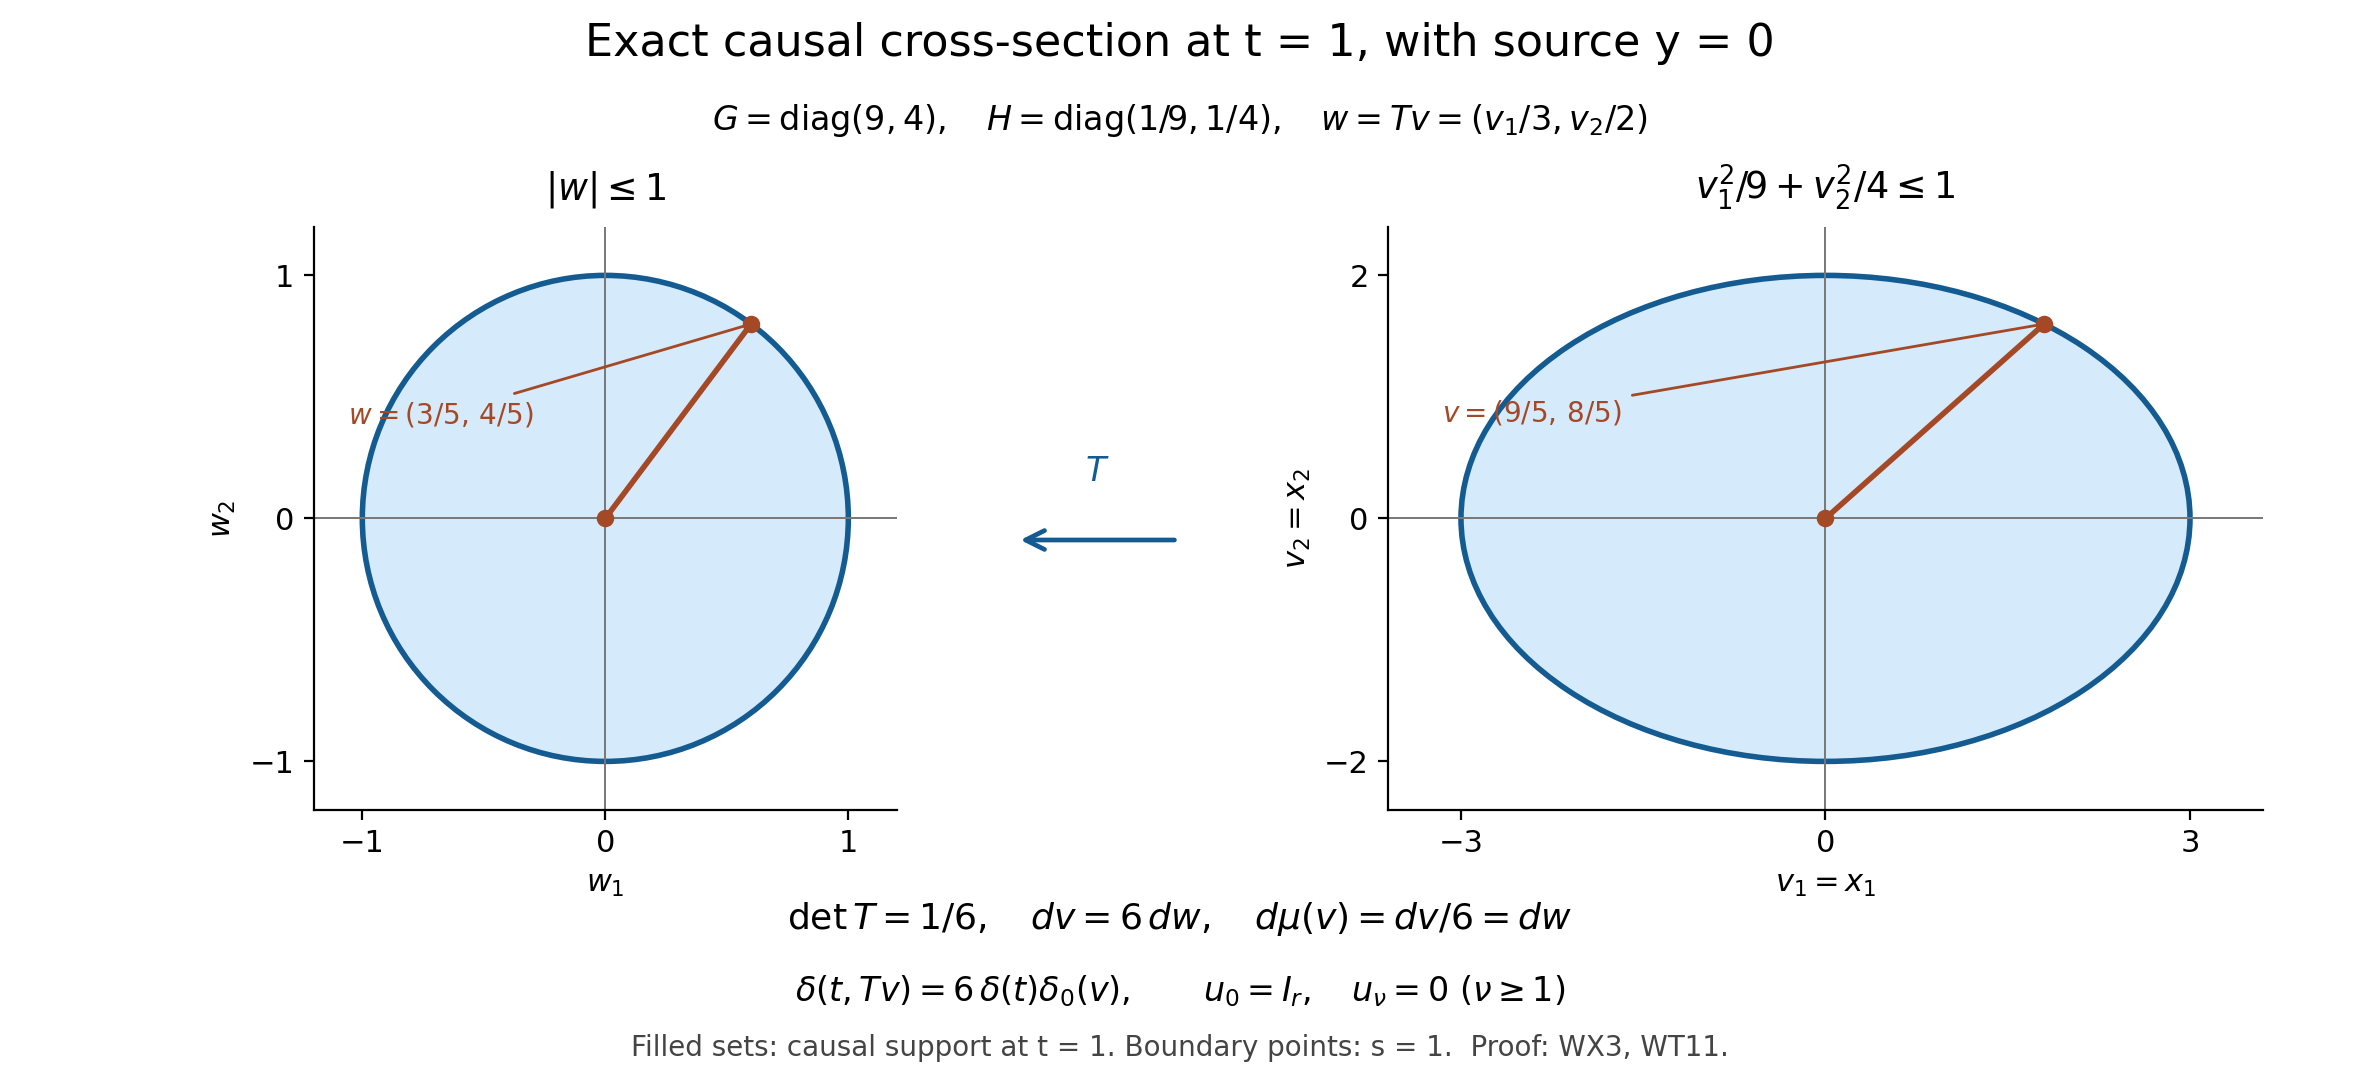
\includegraphics[keepaspectratio,alt={Exact causal ellipse and its full density map for the constant metric in WX3}]{../figures/wave-causal-density.png}}
\caption{Exact causal ellipse and its full density map for the constant
metric in WX3}
\end{figure}

The figure uses the original example \(G=\operatorname{diag}(9,4)\),
\(y=0\), \(t=1\), and the exact map \(w=(v_1/3,v_2/2)\). The marked
boundary points are \(w=(3/5,4/5)\) and \(v=(9/5,8/5)\), both of
distance one; the full coordinate Jacobian is six. The density and
point-source factors are those proved in (WT11) and (WG18). The filled
ellipse is a support cross-section, not a plot of a finite value at its
singular boundary. \href{../figures/wave-causal-density.py}{Reproducible
script} and \href{../figures/wave-causal-density.svg}{vector figure}.

\textbf{A constant matrix potential keeps its order in the expansion.}
Let \(P=-\Delta I_r+C\), with any fixed complex matrix \(C\). Then
\(h=0\), \(u_0=I_r\), and (WG5) gives \[
 u_\nu=\frac{(-C)^\nu}{\nu!},\qquad
 (\partial_t^2+P)\sum_{\nu=0}^N\frac{(-C)^\nu}{\nu!}E_\nu
  =\delta I_r+\frac{(-1)^NC^{N+1}}{N!}E_N.
 \tag{WX4}
\] The formula follows by induction: the transport equation for a
constant amplitude is \(\nu u_\nu=-Cu_{\nu-1}\). No diagonalization,
real eigenvalues or positivity are used. If \(C^m=0\), the finite sum
with \(N=m-1\) is already an exact causal fundamental kernel, since the
displayed remainder vanishes.

\subsubsection{13.1. A complete consequence for every constant complex
potential}\label{a-complete-consequence-for-every-constant-complex-potential}

The nilpotent example has a further consequence at its original matrix
generality. For any constant complex \(r\)-by-\(r\) matrix \(C\), every
spatial dimension \(n\geq1\), and the original operator
\(\partial_t^2-\Delta_x I_r+C\), the full original sum \[
 K_C(t,x)=\sum_{\nu=0}^\infty
                      \frac{(-C)^\nu}{\nu!}E_\nu(t,x)
 \tag{WK1}
\] converges as a causal spacetime distribution, and on positive time
with all one-sided derivatives into tempered spatial distributions. It
is an exact fundamental kernel, with zero initial value and first
derivative \(\delta_0I_r\). This extends the finite nilpotent
calculation; it is not an assertion that an infinite geometric Hadamard
series converges for variable coefficients.

To prove it, retain the simplex formula (W22). Its nonnegative weight
has integral (W23), and each derivative of
\(\sin z/z=\int_0^1\cos(sz)\,ds\) of order \(m\) is bounded on the real
line by \(1/(m+1)\). For \(T\geq1\), the full product rule therefore
gives, for every \(j\geq0\), \[
 \left\|\partial_t^j\left(
               \frac{(-C)^\nu}{\nu!}h_\nu(t,\omega)\right)\right\|
 \leq D_j\frac{\|C\|^\nu}{\nu!}\,\nu!\,
       \frac{(2\nu+1)^{2j}T^{2\nu+1}}{(2\nu+1)!}
       (1+\omega)^j,\qquad 0\leq t\leq T.
 \tag{WK2}
\] For the derivative on the power \(t^{2\nu+1}\), keep its falling
product and its remaining nonnegative power; only orders through
\(2\nu+1\) can occur. The other derivatives have at most \((\nu+1)^j\)
labeled product assignments, each with its actual factors
\((\omega u_i)^m\). Since \(0\leq u_i\leq1\), their absolute integrals
are bounded by the original weight integral (W23). The finite binomial
sum of the two derivative types is bounded by the displayed polynomial
in \(2\nu+1\), with a constant depending only on \(j\). This proves
(WK2), including \(\omega=0\) and \(\nu=0\); the two factorial factors
from the original amplitude and original \(E_\nu\) are displayed before
their numerical comparison.

The sum of the coefficients on the right converges: after their exact
factorial cancellation, its successive ratio tends to zero, because the
denominator contributes \((2\nu+3)(2\nu+2)\) and its numerator has only
the fixed polynomial ratio and \(\|C\|T^2\). Pairing the retained
polynomial frequency bound against any Schwartz test proves uniform
convergence with every fixed time derivative, uniformly over bounded
sets of Schwartz tests. The fundamental theorem and the same convergent
bounds justify differentiation of the sum. Integrating such a pairing
against a compact spacetime test, with its spatial Schwartz seminorms
uniformly bounded in time, proves convergence as a spacetime
distribution. Every partial sum is supported in \(C_+\); testing outside
that closed cone and passing to the limit proves the same support for
the sum.

For the partial sum through \(N\), (WX4) gives its full error \[
 \frac{(-1)^N}{N!}C^{N+1}E_N.
 \tag{WK3}
\] Its tested absolute bound is the right side of (WK2) at \(j=0\), with
\(\|C\|^\nu\) replaced by \(\|C\|^{N+1}\), and tends to zero on every
compact time interval. Differential operators are continuous on
distributions by their transposed test seminorms, so the complete finite
identities pass to \[
 (\partial_t^2-\Delta_x I_r+C)K_C
                 =\delta(t)\delta_0(x)I_r.
 \tag{WK4}
\] The uniform derivative convergence and (W19) give both initial data.
On positive time the point source vanishes, so repeated use of the
original differential equation gives every further jet, retaining its
entire binomial expansion: \[
\begin{split}
 \partial_t^{2m}K_C(0+,\cdot)&=0,\\
 \partial_t^{2m+1}K_C(0+,\cdot)
    &=(-1)^m\sum_{\ell=0}^m
       \binom m\ell C^\ell(-\Delta_x)^{m-\ell}\delta_0\,I_r .
\end{split}
 \tag{WK5}
\] Here \(m\geq0\), and the \(\ell=0\) matrix power is the original
identity. Scalar spatial derivatives commute with the constant \(C\),
which proves that expansion; no commutation of variable matrix
coefficients is inferred.

These data determine the evolution in the class of twice continuously
differentiable tempered-distribution-valued solutions. Indeed Fourier
transformation gives the original matrix polynomial \(|\xi|^2I_r+C\).
For a solution difference \(u\) with zero initial data and a terminal
time \(T\), choose a smooth compact frequency test \(\psi\). The
backward matrix equation \(v''+(|\xi|^2I_r+C)^t v=0\), with
\(v(T)=0,\ v'(T)=\psi\), has a smooth compactly supported test solution:
the ordered finite-dimensional flow theorem NF6--NF11 applies on the
compact frequency support, with all parameter derivatives, and the
initial test factor keeps that same support. The exact bilinear
distribution pairing has constant Wronskian \[
 \frac{d}{dt}\big(\langle u',v\rangle-\langle u,v'\rangle\big)
       =\langle-(|\xi|^2I_r+C)u,v\rangle
           +\langle u,(|\xi|^2I_r+C)^t v\rangle=0 .
 \tag{WK6}
\] Its initial value is zero and its terminal value is
\(-\langle u(T),\psi\rangle\), so \(u(T)=0\). Transpose is used because
this is the bilinear distribution pairing; introducing a conjugate would
change that convention. Arbitrary \(T\) and arbitrary compact tests
prove uniqueness. Schwartz continuity then gives uniqueness as tempered
distributions too.

The smaller finite-order odd receiver from (WT12) also propagates to
this exact sum. Define \(W_C=K_C-\widetilde K_C\). Choose one integer
\(k\geq0\) with \(k\geq(n-1)/2\); it satisfies (OE18) for every index.
The finitely many indices with \(a_\nu<0\) have the bounds already
proved. For all larger indices, (OE8) and (OE15) give, on tests
supported in \([-R,R]\) with \(R\geq1\), \[
\begin{split}
 |\langle W_\nu,\phi\rangle|
   &\leq |A_\nu|\frac{4R^{2a_\nu+1}}{\Gamma(a_\nu+1)}
                         \|\phi\|_\infty,\\
 |\langle\partial_tW_\nu,\phi\rangle|
   &\leq |A_\nu|\frac{2R^{2a_\nu}}{\Gamma(a_\nu+1)}
                         \|\phi\|_\infty .
\end{split}
 \tag{WK7}
\] These estimates are uniform in \(|x|^2\) on compact sets; tests
outside the cone simply pair to zero. Multiplication by the original
amplitude norm \(\|C\|^\nu/\nu!\) gives a summable majorant, whose
successive ratio has the two growing factors \(\nu+1\) and \(a_\nu+1\)
in its denominator. The finite low-index bounds and this uniform tail
prove weak continuity of \(x\mapsto W_C(\cdot,x)\) into order \(2k-1\)
when \(k\geq1\), and of its time derivative into order \(2k\). For
\(k=0\) both valid bounds are order zero. The entire series agrees off
the center with the spacetime odd difference by its tested convergence
and agrees at the center by that continuity. In odd spatial dimension
\(n\geq3\), choosing \(k=(n-1)/2\) makes the primitive bound sharp: the
zeroth term has a nonzero \(I_r\delta^{(n-2)}\) coefficient by (OE19),
while every subsequent exceptional term has lower derivative order and
the remaining tail has order zero. The scaled test used after (WT12)
makes the leading term grow as \(\epsilon^{-1}\) and all those
lower-order terms stay bounded. This sharpness assertion concerns
positive rank; rank zero has the empty kernel. The source factors and
all higher-index contributions remain in (WK1).

\subsection{14. Problems and complete
solutions}\label{problems-and-complete-solutions}

\textbf{Problem 1 --- The first three initial traces in one dimension.}
Compute \(E_1\) for \(n=1\), integrate it against a smooth spatial test,
and verify the first nonzero initial derivative.

\textbf{Solution.} Here \(a=1\), \(A_1=1/8\), so
\(E_1(t,x)=\boldsymbol1_{\{t>0\}}(t^2-x^2)_+/8\). At \(t>0\),
substitution \(x=tu\) gives \[
 \langle E_1(t,\cdot),\phi\rangle
     =\frac{t^3}{8}\int_{-1}^{1}(1-u^2)\phi(tu)\,du
     =\frac{t^3}{6}\phi(0)+O(t^5).
 \tag{WP1}
\] The odd Taylor term integrates to zero, and the remainder bound
follows from the second derivative of \(\phi\) on a fixed compact
interval. Smoothness in \(t\geq0\) follows by differentiating the fixed
integral. Derivatives of orders zero, one and two vanish at zero; the
third derivative is \(\phi(0)\). Thus the trace is \(1!\delta_0\), with
the exact normalization.

\textbf{Problem 2 --- Why the test order cannot be lowered.} At
\(n=5,\nu=0\), find \(\partial_tW_0(t,0)\), and show that a uniform
order-three estimate cannot hold near \(x=0\).

\textbf{Solution.} Now \(k=2\), \(a=-2\), and (OE19) gives \[
                       \partial_tW_0(t,0)=\frac1{12\pi^2}\delta^{(4)}(t).
 \tag{WP2}
\] Indeed \(2^{2k-n+1}=1\) and \(k!/(2k)!=1/12\). If an order-three
estimate uniform near \(x=0\) held, continuity on smooth tests would
pass that estimate to \(x=0\). Choose \(\psi\in C_c^\infty\) with
\(\psi^{(4)}(0)\ne0\), and let
\(\phi_\varepsilon(t)=\varepsilon^3\psi(t/\varepsilon)\). Its
derivatives through order three stay bounded on one fixed support, but
the pairing with (WP2) grows as \(\varepsilon^{-1}\). This contradiction
proves the claim.

\textbf{Problem 3 --- Weak convergence is not norm convergence.} For
\(e_{\delta,0}\), compute its distance from \(e_{0,0}\) in total
variation and its limit against a continuous test.

\textbf{Solution.} For \(\delta>0\), the three support points
\(\sqrt\delta,-\sqrt\delta,0\) are distinct. The signed difference has
masses \(1,1,-2\), so its total variation is \(4\). On a continuous test
\(\phi\), its value is
\(\phi(\sqrt\delta)+\phi(-\sqrt\delta)-2\phi(0)\), which tends to zero
by continuity at the origin. These facts hold even on a fixed interval
containing all points for small \(\delta\). They explain precisely why
the topology in Section 6 was specified on fixed \(C^m\) tests.

\textbf{Problem 4 --- Design an error with three continuous
derivatives.} In spatial dimension \(n=4\), choose the smallest
truncation index guaranteed by this lesson to give a \(C^3\) remainder
for arbitrary smooth coefficients. Explain what fails at the next
smaller index.

\textbf{Solution.} Inequality (WG14) reads \(3<N-3/2\), hence the
smallest integer is \(N=5\). For \(N=4\), the exponent of the cone power
is \(a=5/2\). At a nonzero cone point its third transverse derivative is
a nonzero constant times \(q_+^{-1/2}\) and is unbounded. If
\(P=-\Delta+1\), (WX4) makes the remainder amplitude a nonzero constant,
so this failure actually occurs. At \(N=5\), \(a=7/2>3\), and Section 11
controls the cone and its vertex.

\textbf{Problem 5 --- A nilpotent system with an exact finite answer.}
Let \[
 C=\begin{pmatrix}0&2&0\\0&0&3\\0&0&0\end{pmatrix},
 \qquad P=-\Delta I_3+C.
 \tag{WP3}
\] Find a causal fundamental kernel and its first initial traces.

\textbf{Solution.} Matrix multiplication gives \(C^2_{13}=6\), every
other entry of \(C^2\) zero, and \(C^3=0\). Formula (WX4) with \(N=2\)
therefore yields \[
 K=E_0I_3-CE_1+\tfrac12C^2E_2
   =\begin{pmatrix}E_0&-2E_1&3E_2\\0&E_0&-3E_1\\0&0&E_0\end{pmatrix}.
 \tag{WP4}
\] Its causal support follows term by term, and the exact equation is
\((\partial_t^2+P)K=\delta I_3\). From (W19), \(K(0+,\cdot)=0\) and
\(\partial_tK(0+,\cdot)=\delta_0I_3\). Terms with \(E_1,E_2\) start at
orders three and five; they do not alter those initial data. This system
is not diagonalizable, so an argument requiring diagonalization would
miss it.

\textbf{Problem 6 --- A cutoff and the first affected time.} A smooth
function \(\theta(x,y)\) equals one where \(s(x,y)\leq2c\), and its
derivatives are supported where \(s(x,y)>2c\) inside a larger normal
neighborhood. Show that multiplying every amplitude by \(\theta\)
changes no finite wave identity on \(t<2c\). Determine whether the same
conclusion necessarily holds at \(t=2c\).

\textbf{Solution.} Each commutator term from \(P_x\) contains a
derivative of \(\theta\) multiplied by a smooth coefficient, an
amplitude, and a spatial derivative of \(E_\nu\). Distributional
derivatives have support contained in that of \(E_\nu\), namely
\(t\geq s(x,y)\). At every point with \(t<2c<s\), a neighborhood still
satisfies \(t<s\); therefore each such term is zero there. The
difference from the uncut product is zero by the same argument.

Under the stated stronger hypothesis the answer at \(t=2c\) is also yes,
locally near each point of that time slice. At \(s=2c\), the closed
support of each derivative of \(\theta\) is absent from a neighborhood,
because that support lies in the open set \(s>2c\). Hence \(\theta\) is
locally constant there, and its value is one by continuity from
\(s<2c\). At \(s<2c\) it is already one, while at \(s>2c\) causal
support makes the kernel vanish near \(t=2c\). These three cases prove
the local assertion. A single larger time interval would require a
uniform positive gap between the affected region and \(s=2c\); it is not
implied just by local separation over a noncompact set. The basic
extension theorem in Section 11 uses only the open time interval and
needs no such gap.

\subsection{15. Exact comparison with the freely available author
version}\label{exact-comparison-with-the-freely-available-author-version}

The comparison here uses Christian Bär, Nicolas Ginoux and Frank
Pfäffle's original author TeX for
\href{https://arxiv.org/abs/0806.1036v1}{arXiv:0806.1036v1}, §1.2, §1.4
and §§2.1--2.3, and the finite identity (2.13) in §2.4. It imports no
global existence result, infinite-series assertion or proof from a
printed edition. All distribution, transport and finite cancellation
statements receiving this comparison have their proofs in this lesson
and the precise earlier programme proofs already named.

Write \(d=n+1\) for their spacetime dimension, and \(\alpha=2\lambda\)
for their parameter. Their flat coefficient becomes \[
 C(2\lambda,n+1)
  =\frac{2^{1-2\lambda}\pi^{(1-n)/2}}
          {\Gamma(\lambda)\Gamma(\lambda+(1-n)/2)}.
 \tag{WC1}
\] Their quadratic form is the original \(q=t^2-|x|^2\). The future
orientation is increasing \(t\), and their name for that branch is
``advanced.'' Their continuous starting range is
\( \operatorname{Re}\alpha>d\), hence
\(\operatorname{Re}\lambda>(n+1)/2\). Our original integral range in
(W6) is broader, \(\operatorname{Re}\lambda>\max(0,(n-1)/2)\); the full
formulas agree on their intersection. Their definition of the remaining
parameters applies the same wave operator recursively, so the compatible
continuation (W10), tested on every compact smooth function, proves
equality for every parameter, including the point source and exceptional
dimensions. It gives the flat correspondence stated in the references,
without replacing any coefficient.

For the geometric comparison keep the product Lorentzian metric \[
 g_{\rm Lor}=-dt^2+\sum_{j,k}H_{jk}(x)\,dx_j\,dx_k,\qquad
 dV=\rho(x)\,dt\,dx,\qquad \rho=(\det G)^{-1/2}.
 \tag{WC2}
\] Its complete Christoffel expression has zero coefficients whenever a
time index occurs, since the time coefficient is constant, the mixed
entries vanish and the spatial coefficients are independent of time. Its
geodesics therefore have affine time and the original spatial
\(H\)-geodesic. The exponential map at \((0,y)\) is
\((t,v)\mapsto(t,\gamma(v,y))\). Its tangent-volume coordinates
\(w=T(y)v\) have the original determinant \(\det T(y)\), so its volume
distortion is \[
 \mu_y(x)=\frac{\rho(x)J(v,y)}{\rho(y)},\qquad
 x=\gamma(v,y).
 \tag{WC3}
\] In particular the distortion is one at the center. The source
definition in §1.4 pairs the flat Riesz distribution with the
pulled-back test multiplied by this distortion. The full inverse test
Jacobian of (WG6), followed by the normal chart, consequently gives the
exact functional comparison \[
 \big\langle R_+^\Omega(2\nu+2,(0,y)),\phi\big\rangle
     =\frac1{\nu!}\big\langle
              E_\nu(t,s(x,y)),\,\rho(x)\phi(t,x)\big\rangle .
 \tag{WC4}
\] The equality follows directly from their definition, not from their
global theorem: \(\mu_y\det T(y)=\rho(x)J\) retains every factor in the
test substitution. It is first the equality of the original integrals
and then the equality of their entire tested continuations. Here the
domain is the actual common small exponential image, and tests have
compact support inside it. No pullback by distance at the diagonal
occurs.

The matrix lower-order terms also have an exact comparison. Put \[
\begin{split}
 d^j&=b^j+\sum_k g^{kj}\partial_k\log\rho\,I_r,\qquad
 A_j=-\frac12\sum_k H_{jk}d^k,\qquad A_t=0,\\
 \nabla_j&=\partial_j+A_j,\qquad \nabla_t=\partial_t,\\
 \mathcal B_0&=c+\rho^{-1}\sum_{j,k}
                       \partial_j(\rho g^{jk}A_k)
                    +\sum_{j,k}g^{jk}A_jA_k,\\
 \partial_t^2+P&=\Box^\nabla+\mathcal B_0,\qquad
 \Box^\nabla=\partial_t^2-
       \rho^{-1}\sum_{j,k}(\partial_j+A_j)
                              \rho g^{jk}(\partial_k+A_k).
\end{split}
 \tag{WC5}
\] The last product acts on the section to its right; every derivative
acts on both its coefficient and its section. Its first-order
contribution is the original scalar volume drift
\(-g^{kj}\partial_k\log\rho\) and the matrix contribution
\(-2\sum_k g^{jk}A_k=d^j\), whose sum is \(b^j\). Its zeroth-order
contribution is the negative of the two added terms in \(\mathcal B_0\).
Expanding proves the full operator equality in (WC5), with no
commutation of matrices assumed. This is the connection-d'Alembert
convention of their §1.5.

Let \(\Pi(av,y)\) be the ordered parallel matrix along
\(a\mapsto\gamma(av,y)\), with initial value \(I_r\). Its equation is
\(\partial_a\Pi=-A_j(\gamma(av,y))\partial_a\gamma^j(av,y)\Pi\), and its
full solution and inverse are constructed by (WT5). The covariant form
of (WT1) is \(H(\gamma)Cv=C^{-t}H(y)v\). It gives \[
 2\mathcal E\Pi=
 \left[\sum_j(C^{-1}b)^j(H(y)v)_j+
                         \mathcal E\log\rho(\gamma)\,I_r\right]\Pi .
 \tag{WC6}
\] Differentiate (WC3), and retain its two varying logarithmic terms.
The term \(\mathcal E\log\rho(\gamma)\) in (WC6) cancels exactly that
term in the derivative of \(\mu_y^{-1/2}\). The remaining equation is \[
 2\mathcal E(\mu_y^{-1/2}\Pi)
          =h(\mu_y^{-1/2}\Pi),\qquad
          (\mu_y^{-1/2}\Pi)(0,y)=I_r.
 \tag{WC7}
\] The proved uniqueness of (WG4) therefore identifies their zeroth
coefficient with the exact \(S=u_0\).

Their source-point variable is our \(y\), and their receiving variable
is our \(x\); keep that order. Their radial recursion, at the original
TeX labels vaunull and vaukaglatt in §2.2 and repeated in §2.3, has
factor \(-\nu\) in front of its ordered integral. Substitute
\(V_{\nu-1}(y,x)=(\nu-1)!U_{\nu-1}(x,y)\), retain \(\mu_y^{-1/2}\Pi=S\)
and its inverse, and keep the time-independent operator
\(\partial_t^2+P_x\) on the coefficient. The time derivative is zero
there. The exact result is \[
 V_\nu(y,\gamma(v,y))=
   -\nu!S(v,y)\int_0^1 a^{\nu-1}S(av,y)^{-1}
                         (\widetilde Pu_{\nu-1})(av,y)\,da
   =\nu!u_\nu(v,y).
 \tag{WC8}
\] Starting from (WC7) proves this for every index. With (WC4), their
\(V_\nu R_+^\Omega(2\nu+2)\) is consequently our \(U_\nu E_\nu\)
integrated against the full density \(\rho(x)\,dt\,dx\). A differential
operator on this density representation has the exact coordinate
functional action \(\rho(\partial_t^2+P_x)\rho^{-1}\): pairing by the
formal transpose verifies that multiplication by \(\rho\) intertwines it
with our coordinate-volume action. Multiplying (WG17) by \(\rho(x)\)
changes its point coefficient to \(\rho(y)\sqrt{\det G(y)}=1\), while
retaining its entire error \(\rho(x)(P_xU_N)E_N\). Thus their finite
identity (2.13), with truncation index \(N+1\), is exactly (WG17) in
this density representation. Every factorial, volume factor, operator
term and source/receiver order is accounted for. This bounded
author-version comparison claims no global Cauchy evolution and no
convergence of an infinite Hadamard series.

\subsection{References}\label{references}

This lesson obtains the causal constants from a Laplace integral and the
time traces from a Volterra simplex, then treats finite-order
restriction and geometric cancellation separately. The domain
reconciliation in Section 7 is explicit because a negative factorial or
a negative derivative order cannot be inserted into an endpoint
expression outside its domain.

Christian Bär, Nicolas Ginoux and Frank Pfäffle,
\href{https://arxiv.org/abs/0806.1036v1}{\emph{Wave Equations on
Lorentzian Manifolds and Quantization}, arXiv:0806.1036v1}, §§1.2 and
2.1--2.4, compares Lorentzian Riesz distributions and bundle Hadamard
coefficients. Their dimension is spacetime dimension, \(n+1\) here, and
their parameter is \(2\lambda\). They call the future-supported branch
``advanced''; our causal kernel satisfies \(E_\nu=\nu!R_+(2\nu+2)\) in
their flat notation. Proposition 2.3.1 covers normally hyperbolic bundle
operators, and their finite-sum identity (2.13) checks the cancellation.
The finite-order restriction, vertex coefficient, and flat cosine
normalization required here are proved explicitly above.

\subsection{Further questions}\label{further-questions}

Three directions continue the work. \textbf{Quantitative coefficient
dependence:} for a fixed compact center set and a prescribed \(C^k\)
error norm, derive the finite list of coefficient seminorms needed in
the transport and coordinate estimates. The proof supplies bounds but
does not optimize that list. \textbf{From finite parametrices to
evolution:} combine increasing-order causal errors with a suitable local
solution operator to obtain an exact evolution and compare the resulting
kernel with the flat cosine spectral relation. Such a step requires an
existence and uniqueness theorem at the selected coefficient regularity;
the finite identity alone is insufficient. \textbf{Reflection at a
boundary:} construct the reflected exponential map and the boundary
matching amplitudes before imposing Dirichlet or other boundary data. A
cutoff of an interior normal kernel supplies neither the reflected ray
nor a boundary condition.

\end{document}
